%导演区
\documentclass[a4paper,11pt,UTF8]{article}%book,report,letter
\usepackage[table]{xcolor}
\usepackage{ctex}
\usepackage{geometry}
\geometry{a4paper,scale=0.8}
\usepackage{amsfonts}
\usepackage{amssymb}
\usepackage{verbatim}
\usepackage{mathrsfs}
\usepackage[arrow,matrix]{xy}
\usepackage{amsmath,amssymb,amscd,bm,bbm,amsthm,mathrsfs}
\usepackage{amsmath,amscd}
\usepackage{amsfonts,amssymb}
\usepackage{xypic}
\usepackage{indentfirst}
\usepackage{diagbox}
\usepackage{graphicx}
\usepackage{subfig}    %% 子图包
\usepackage{float} 
\usepackage{caption}
\captionsetup{labelfont=bf}
\usepackage{zhnumber} % change section number to chinese
%这下面为在latex中插入代码所需环境
\usepackage{CJK}
\usepackage{listings}
\usepackage{xcolor}
\lstset{
	language=Matlab,  %代码语言使用的是matlab
	frame=shadowbox, %把代码用带有阴影的框圈起来
	rulesepcolor=\color{red!20!green!20!blue!20},%代码块边框为淡青色
	keywordstyle=\color{blue!90}\bfseries, %代码关键字的颜色为蓝色,粗体
	commentstyle=\color{red!10!green!70}\textit,    % 设置代码注释的颜色
	showstringspaces=false,%不显示代码字符串中间的空格标记
	numbers=left, % 显示行号
	numberstyle=\tiny,    % 行号字体
	stringstyle=\ttfamily, % 代码字符串的特殊格式
	breaklines=true, %对过长的代码自动换行
	extendedchars=false,  %解决代码跨页时,章节标题,页眉等汉字不显示的问题
	texcl=true}
\def\d{\textup{d}}

\theoremstyle{plain}
\newtheorem{thm}{定理}[section]
\newtheorem{lem}{引理}[section]
\newtheorem{prop}{命题}[section]
\newtheorem{cor}{推论}[section]


\renewcommand{\qedsymbol}{$\square$}
\renewcommand\baselinestretch{1.25}
\renewcommand\thesection{\zhnum{section}}
\renewcommand \thesubsection {\arabic{section}}
%正文区
\begin{document}
	\title{\heiti 课题组组会-练习2}
	\author{王程 }
	\date{\today}
	\maketitle
	
	\section{练习及结果}
	1.已知方程组$Ax=b$,其中$A\in \mathcal{R}^{20\times20}$,定义为
	\begin{equation*}
		\begin{bmatrix} 
			3 & -1/2 & -1/4 & \\
			-1/2 & 3 & -1/2 & -1/4\\
			-1/4 & -1/2 & 3 & -1/2& \ddots\\
			     & \ddots & \ddots & \ddots &\ddots& -1/4\\
			     &        & -1/4&-1/2 & 3 & -1/2\\
			     &    &   & -1/4 &-1/2 &3
		\end{bmatrix}
	\end{equation*}
试通过迭代法求解此方程组,认识迭代法收敛的含义以及迭代初值和方程组系数矩阵性质对收敛速度的影响。\\
\indent 实验要求:\\
	\indent(1)选取不同的初始向量$x^{\left(0\right)}$和不同的方程组右端项向量$b$,给定迭代误差要求,用雅克比迭代法和高斯-赛德尔迭代法计算,观测得到的迭代向量序列是否收敛?若收敛,记录迭代次数,分析计算结果并给出你的结论。\\
	\indent(2)取定右端向量$b$和初始向量$x^{\left(0\right)}$,将$A$的主对角线元素成倍增长若干次,非主对角线元素不变,每次用雅克比迭代法计算,要求迭代误差满足$||x^{\left(k+1\right)}-x^{\left(k\right)}||_{\infty}<10^{-5}$,比较收敛速度,分析现象,并得出你的结论。\\
	\indent(3)取定右端向量$b$和初始向量$x^{\left(0\right)}$,分别使用$a$)高斯-赛德尔迭代,$b$)对称高斯-赛德尔迭代,$c$)对以上两种方法分别加上松弛因子$\omega$进行求解,比较收敛速度,分析现象,得出结论。 \\
	~\\


	\textbf{解:}\\
	\indent(1)采用随机数生成的方法构建初始向量$x^{\left(0\right)}$,$x^{\left(0\right)}$中的元素为$0\sim{1}$之间的随机数。同样的,采用随机数生成的方法构建右端项向量$b$,$b$中的元素为$0\sim{100}$之间的随机数,要求迭代误差满足$||x^{\left(k+1\right)}-x^{\left(k\right)}||_{\infty}<10^{-5}$。以下分别给出两种迭代法的迭代次数与误差量级变化图,其中高斯-赛德尔迭代分别采用了Forward sweep 和 Backward sweep。
	\newpage
	\textbf{雅克比迭代法}
		\begin{figure}[!h]
		\centering
		\subfloat[random1]{
			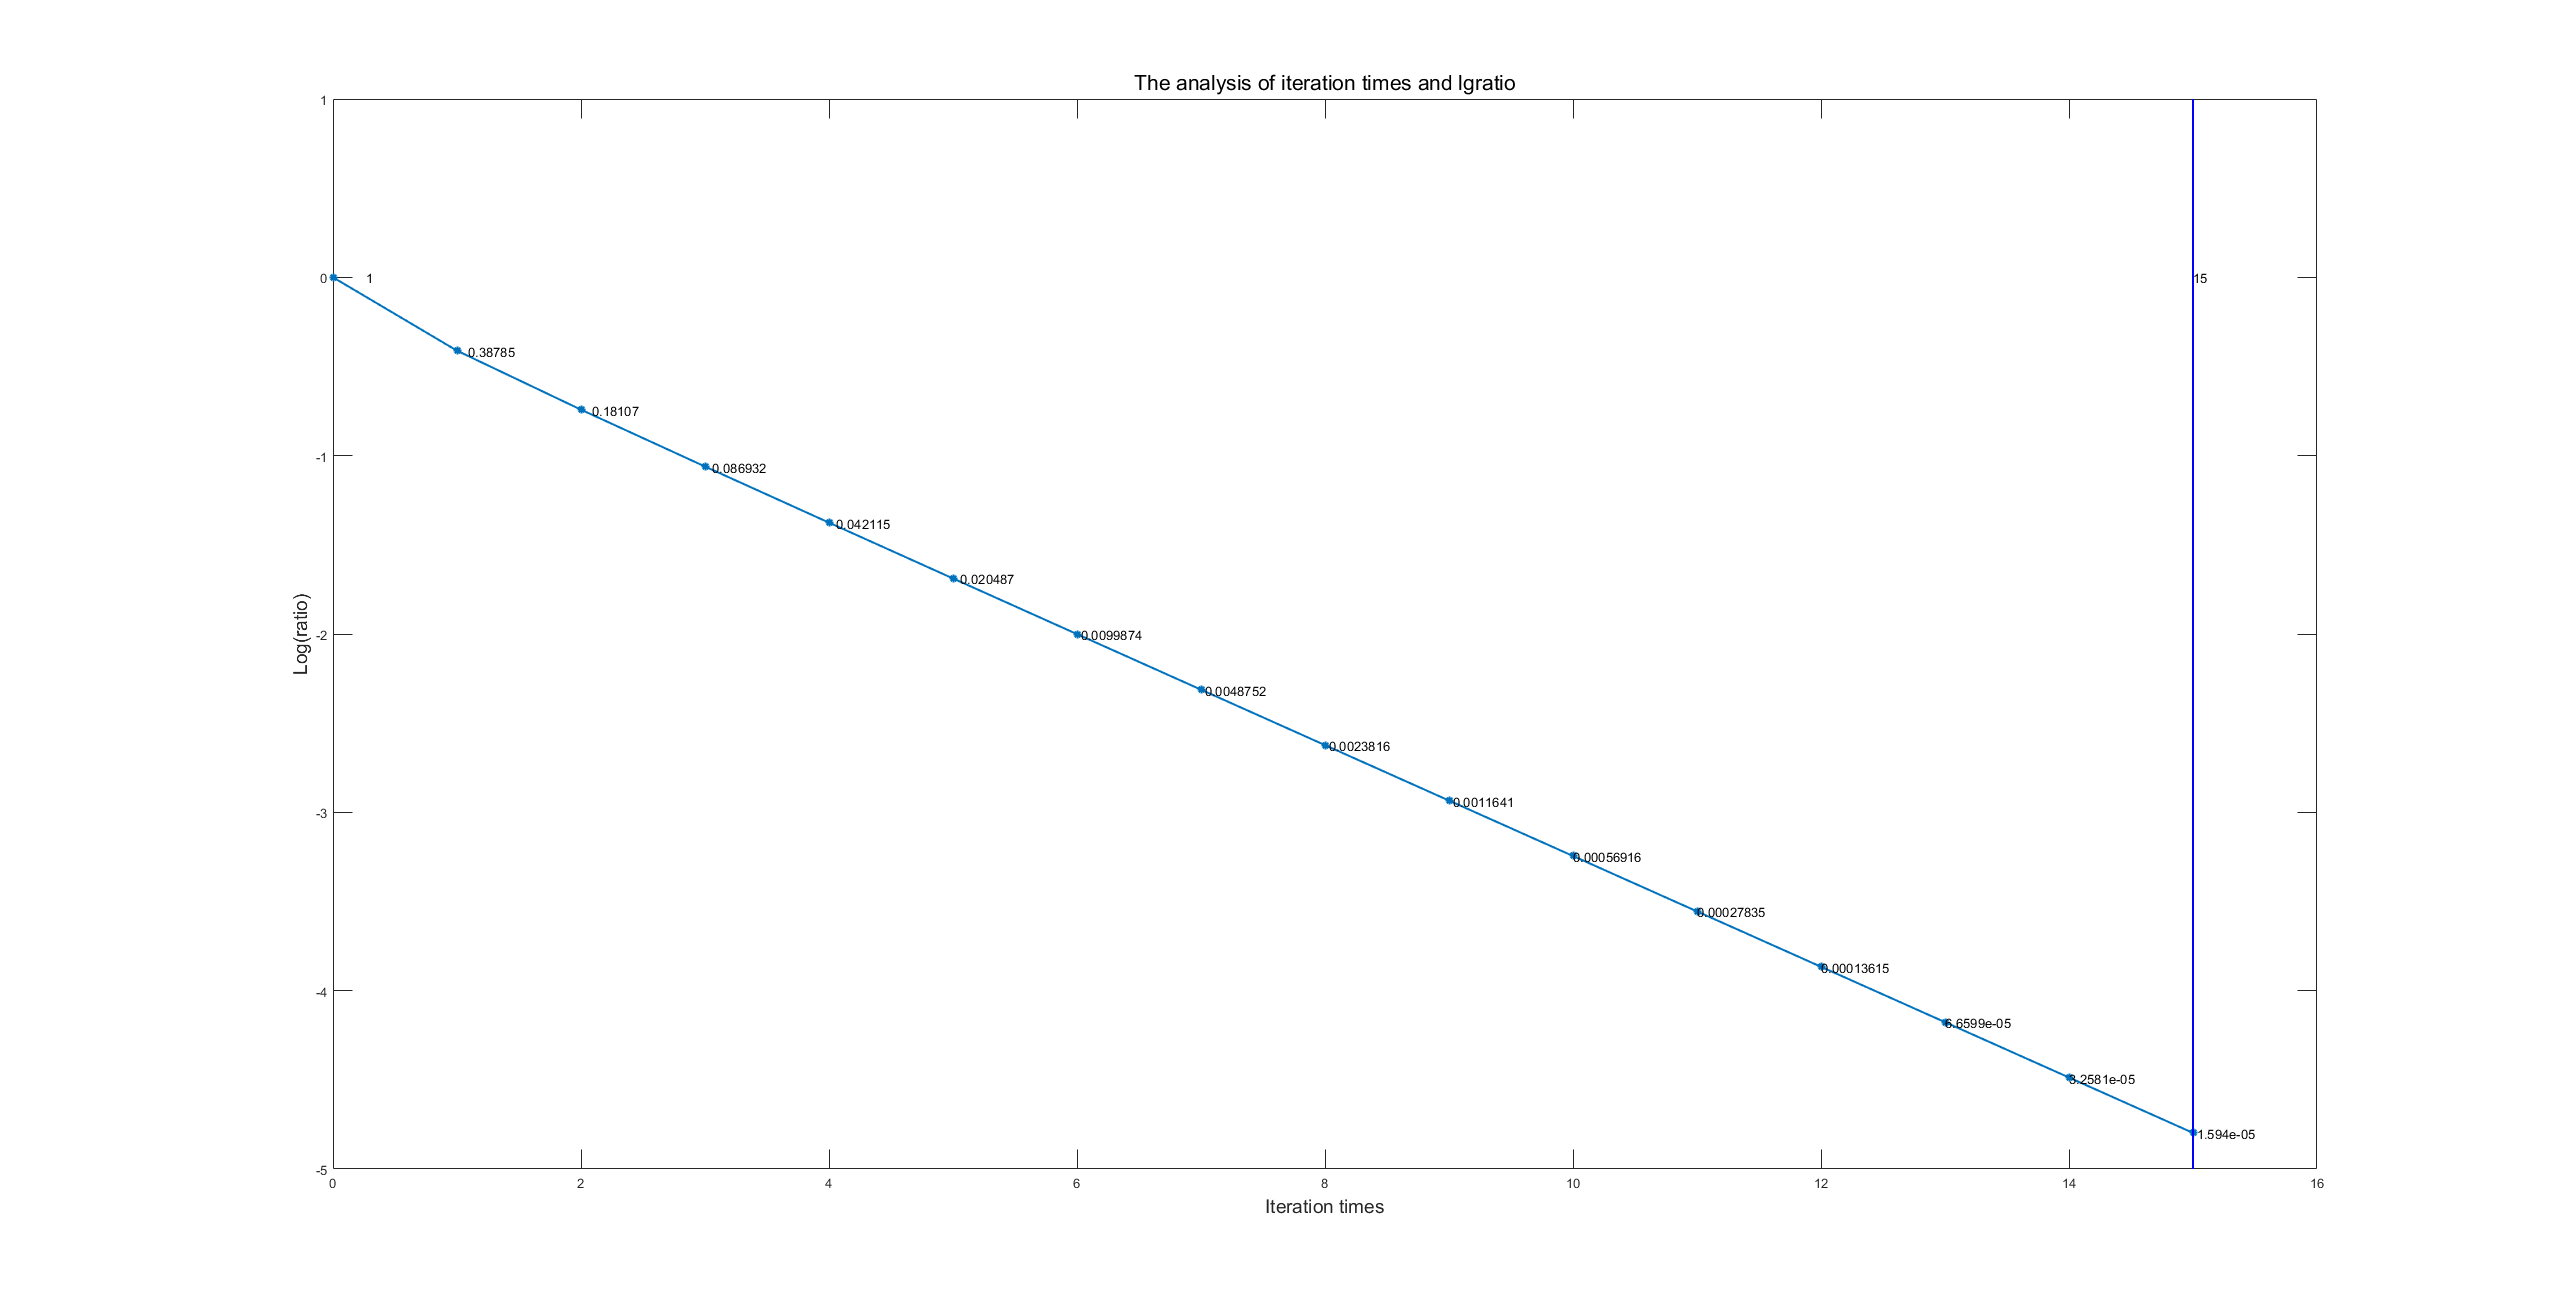
\includegraphics[width=3in]{Jacobi迭代-tol=10^(-5)rand1.png} 
		}
		\hfill
		\subfloat[random2]{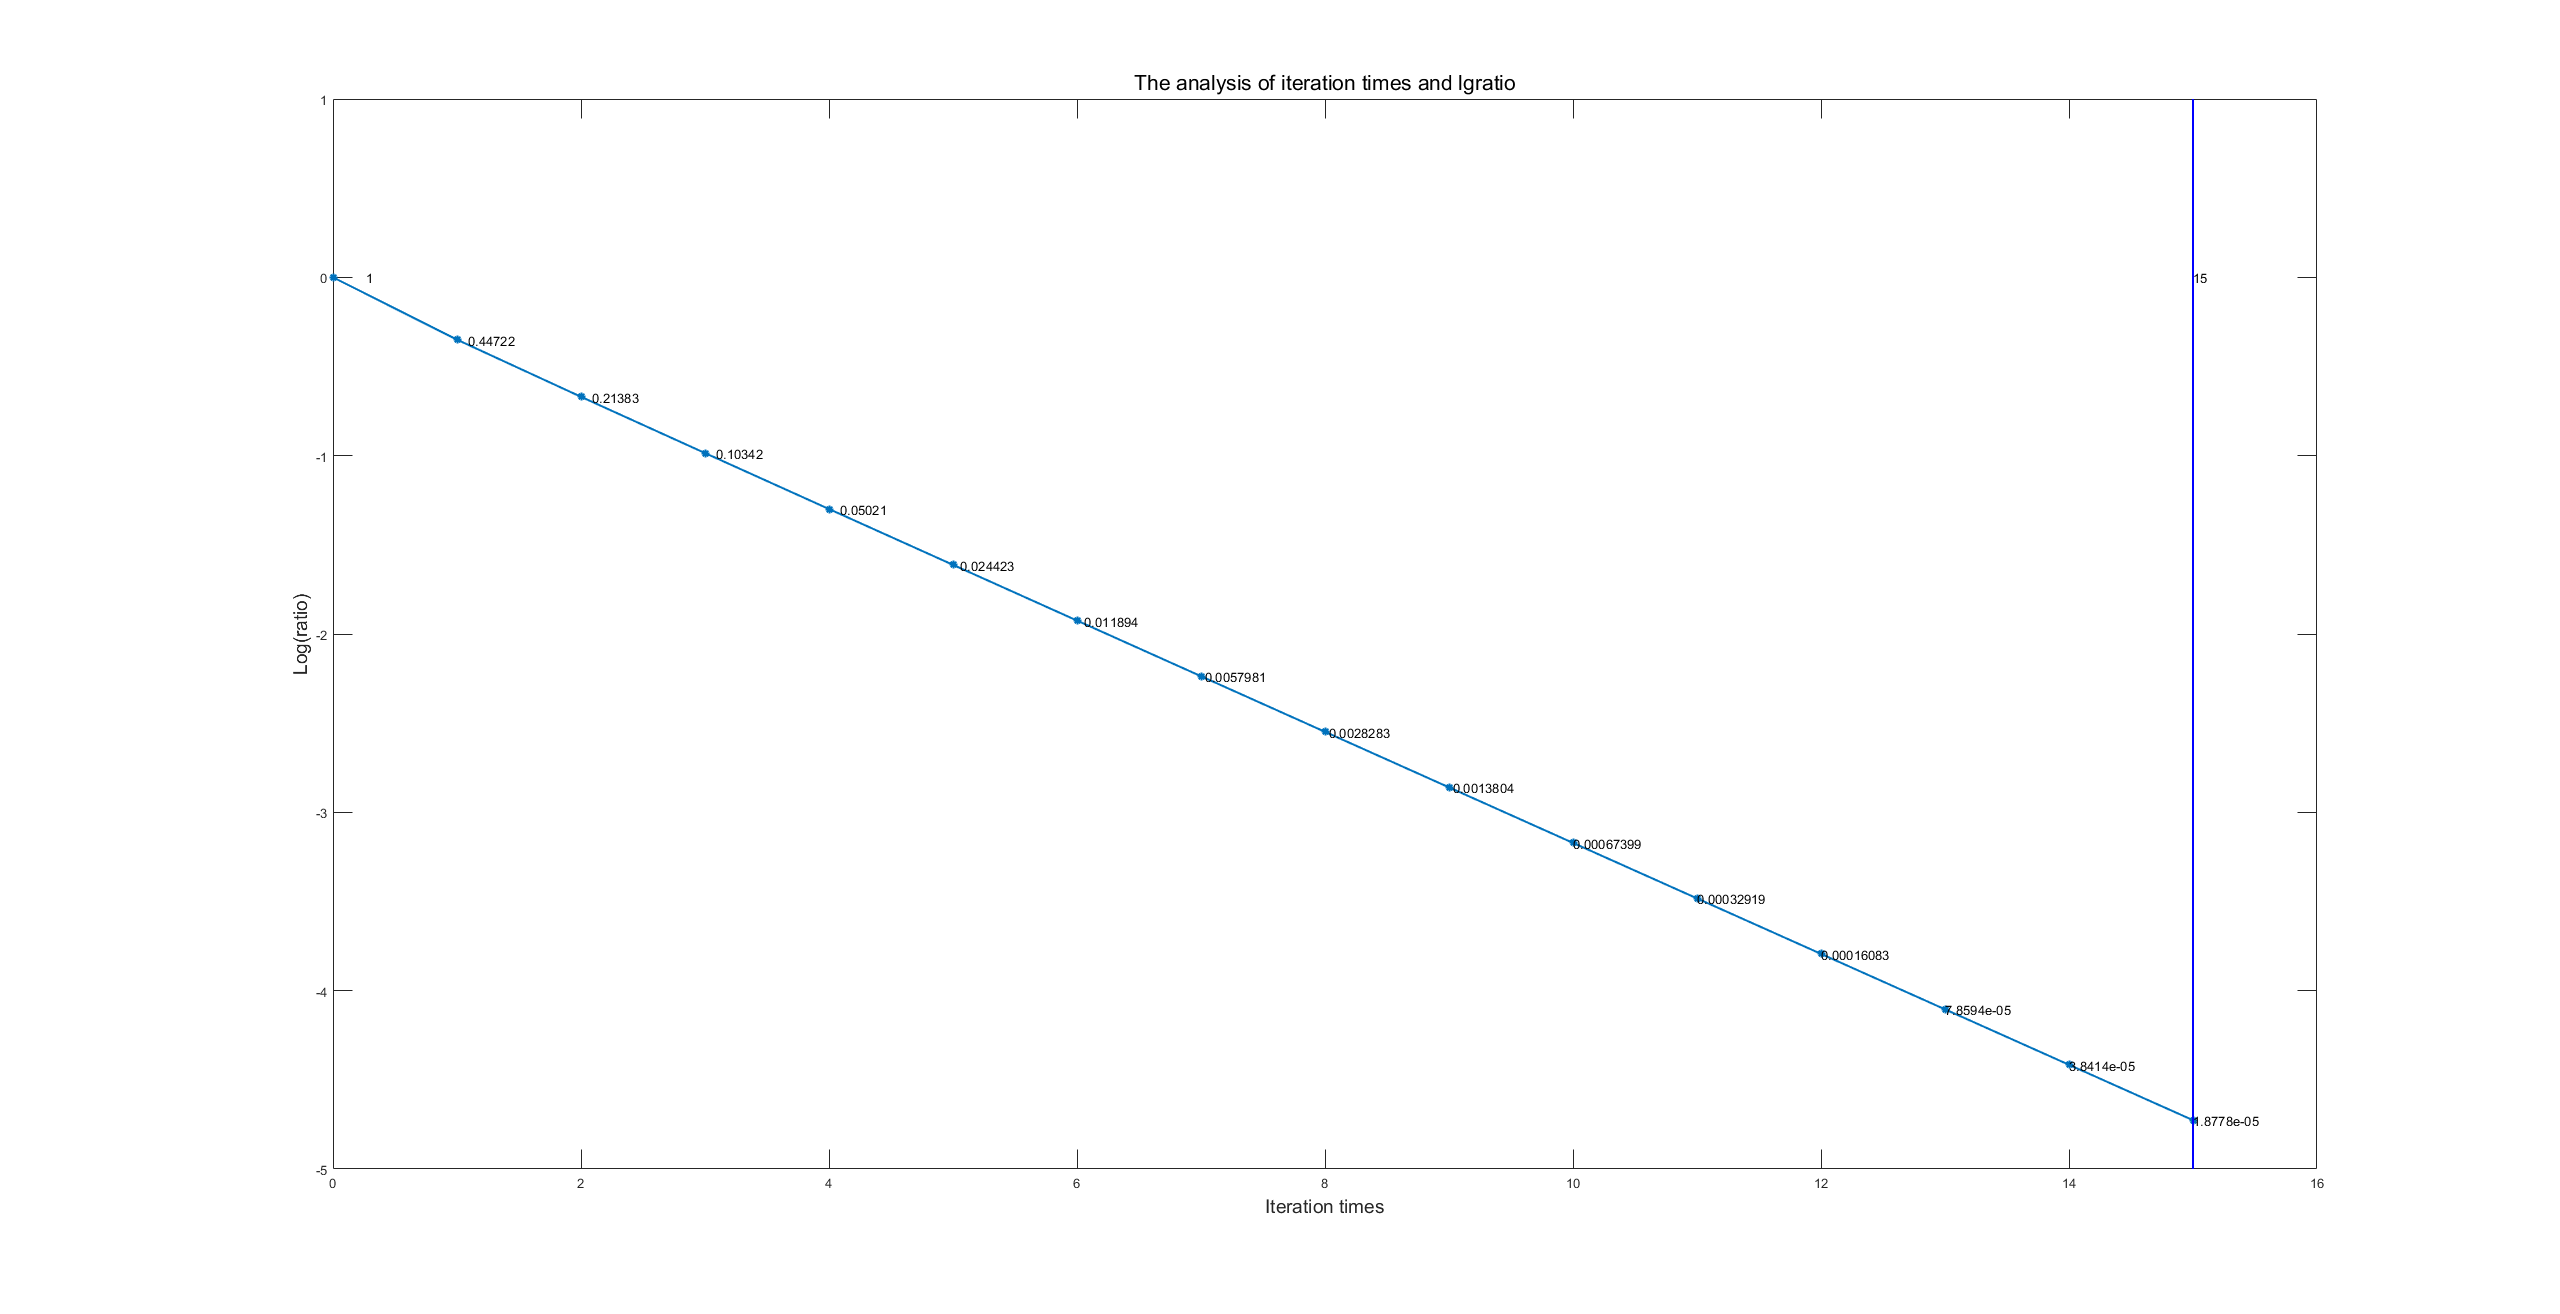
\includegraphics[width=3in]{Jacobi迭代-tol=10^(-5)rand2.png} }
		\newline
		\subfloat[random3]{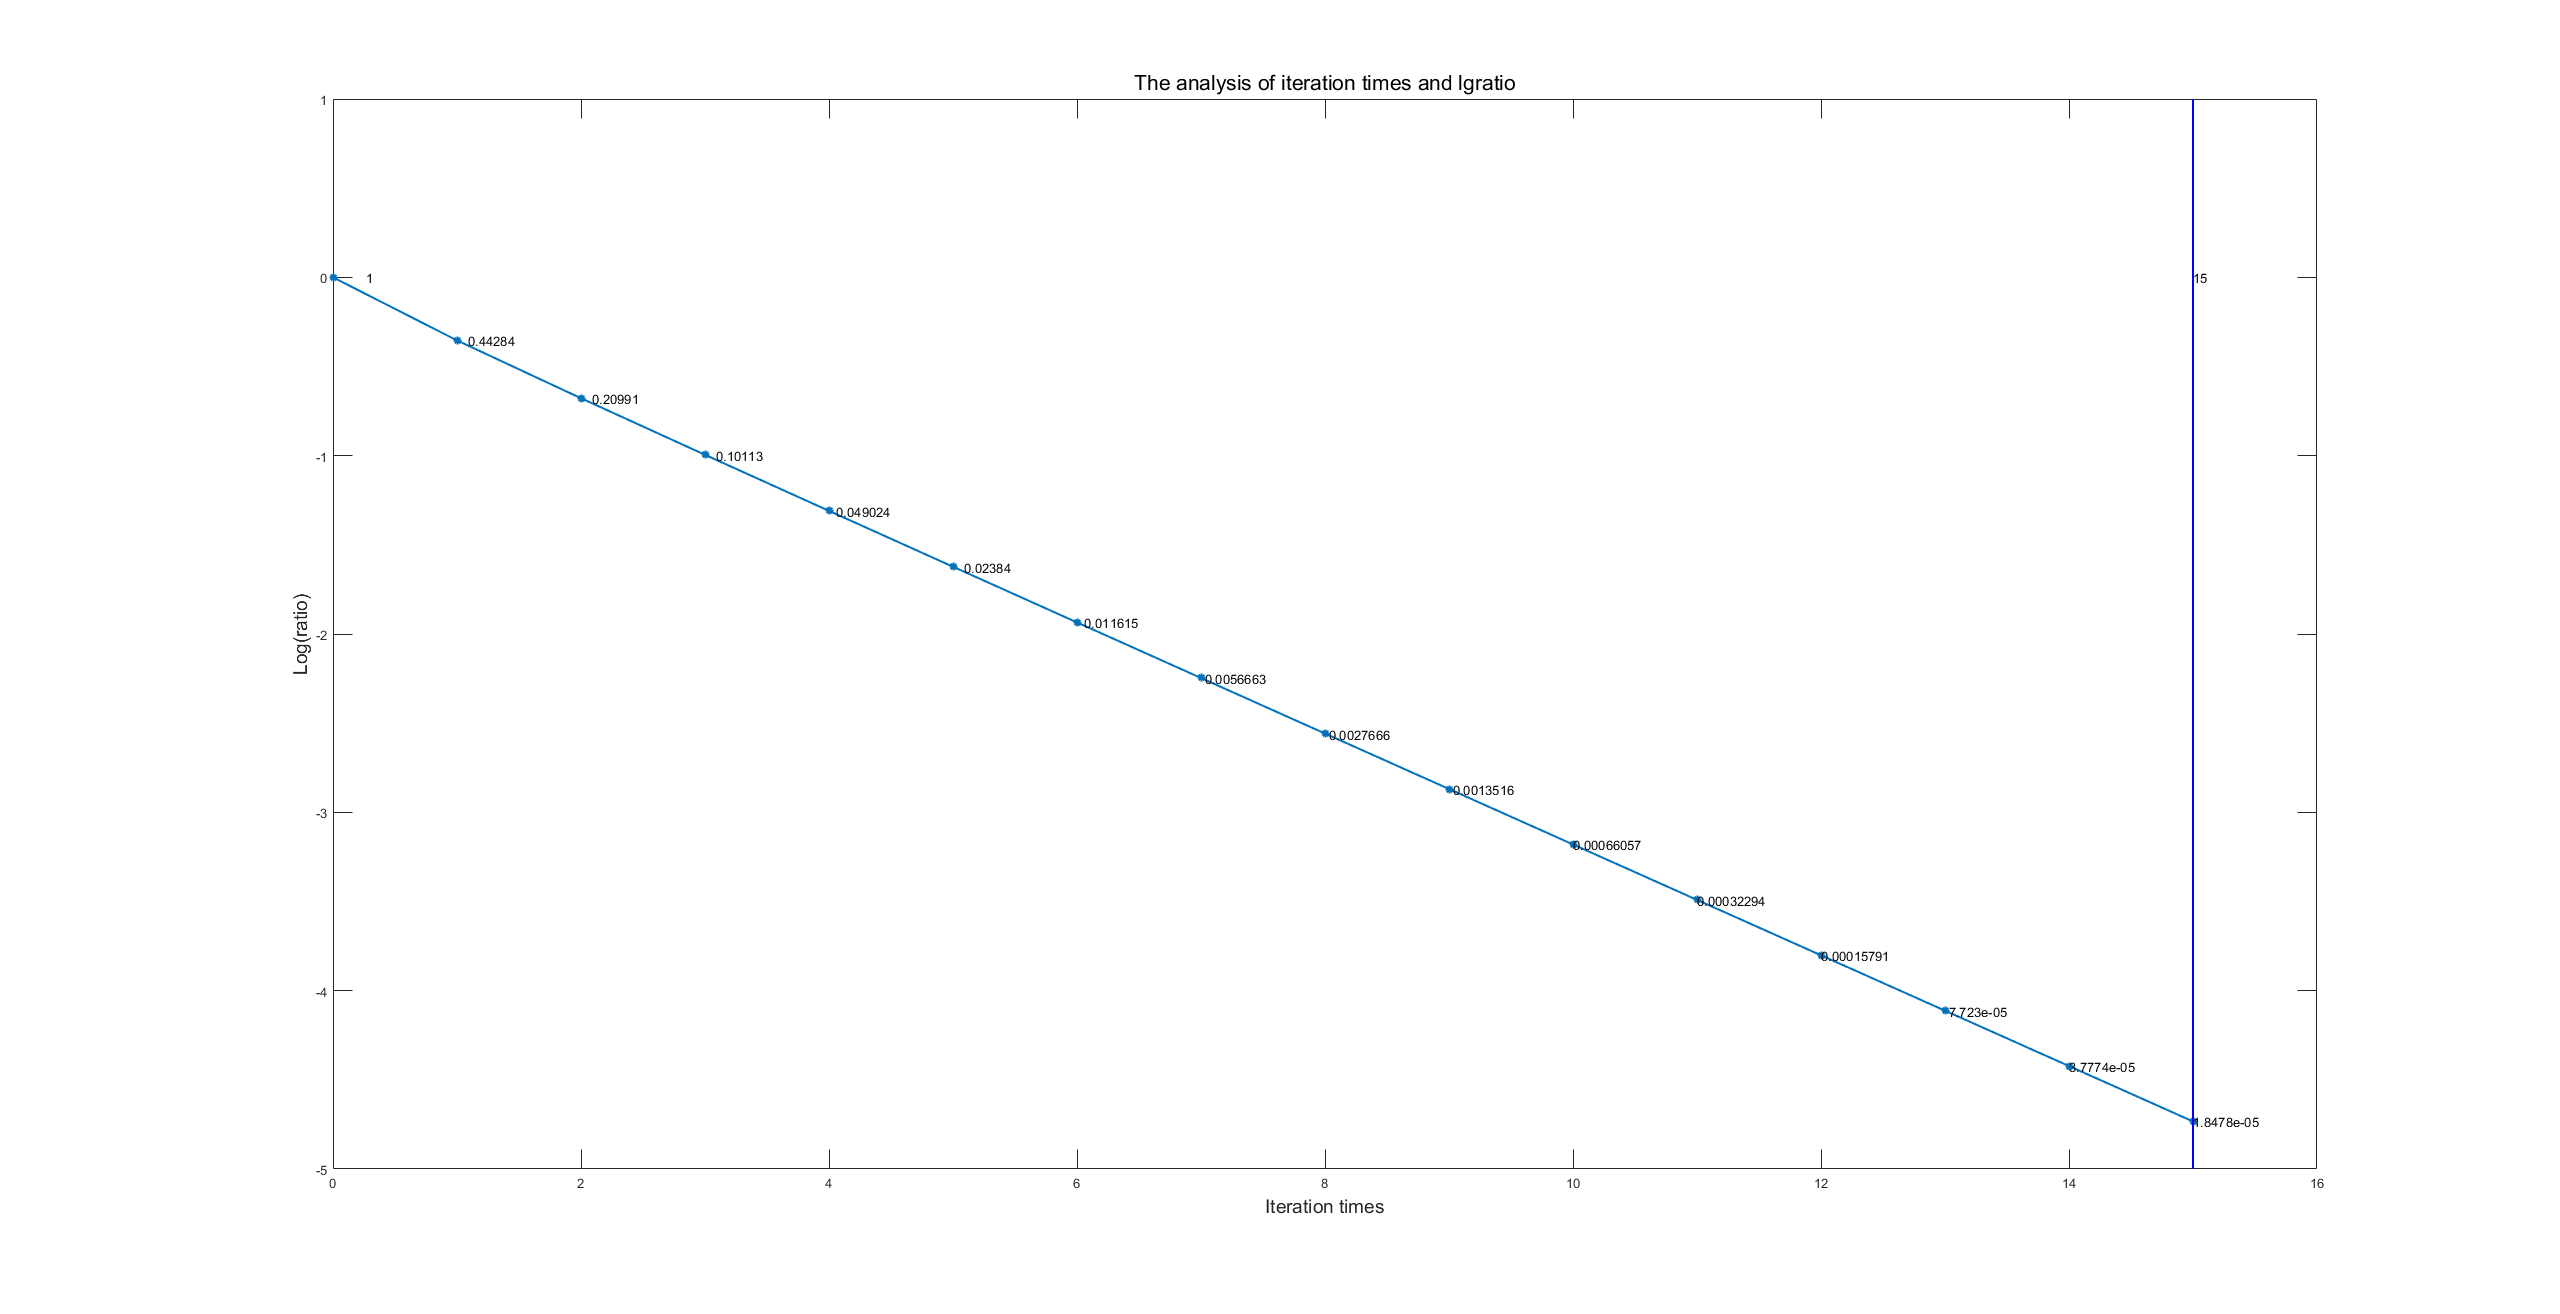
\includegraphics[width=3in]{Jacobi迭代-tol=10^(-5)rand3.png} }
		\hfill
		\subfloat[random4]{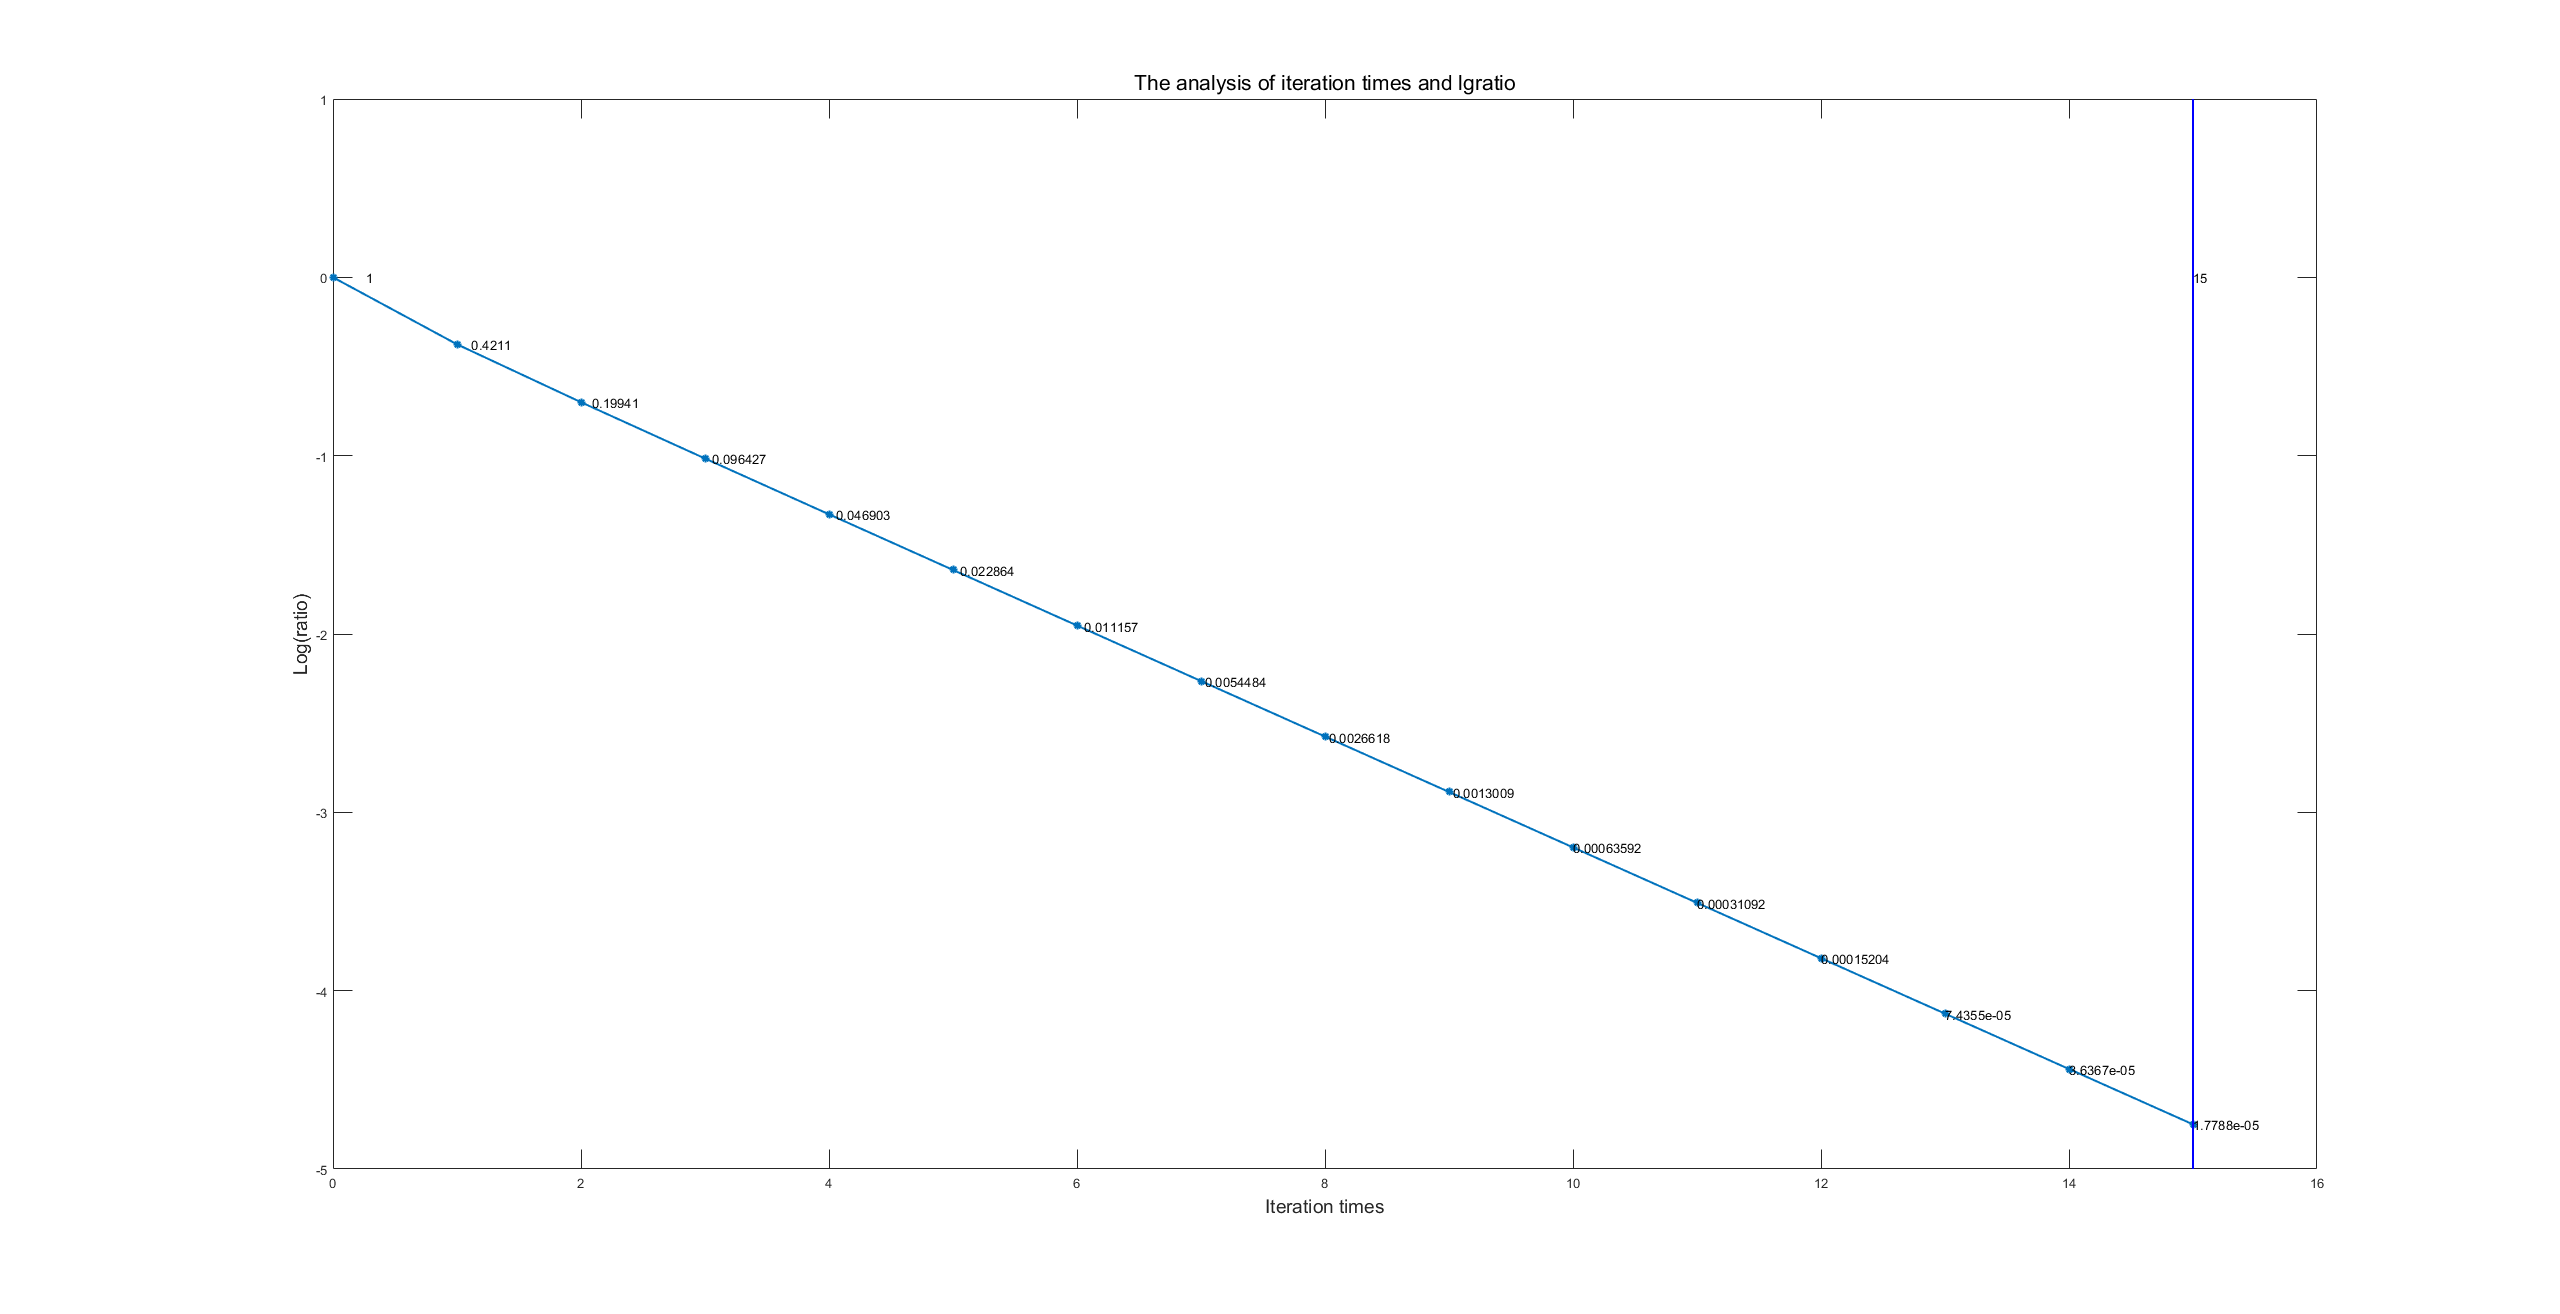
\includegraphics[width=3in]{Jacobi迭代-tol=10^(-5)rand4.png} }	
		\caption{雅克比迭代次数和误差量级图}
	\end{figure}\\
%	\vspace{10pt}\\
	\indent \textbf{高斯-赛德尔迭代法}\\
	\begin{figure}[!h]
		\centering
		\subfloat[random1]{
			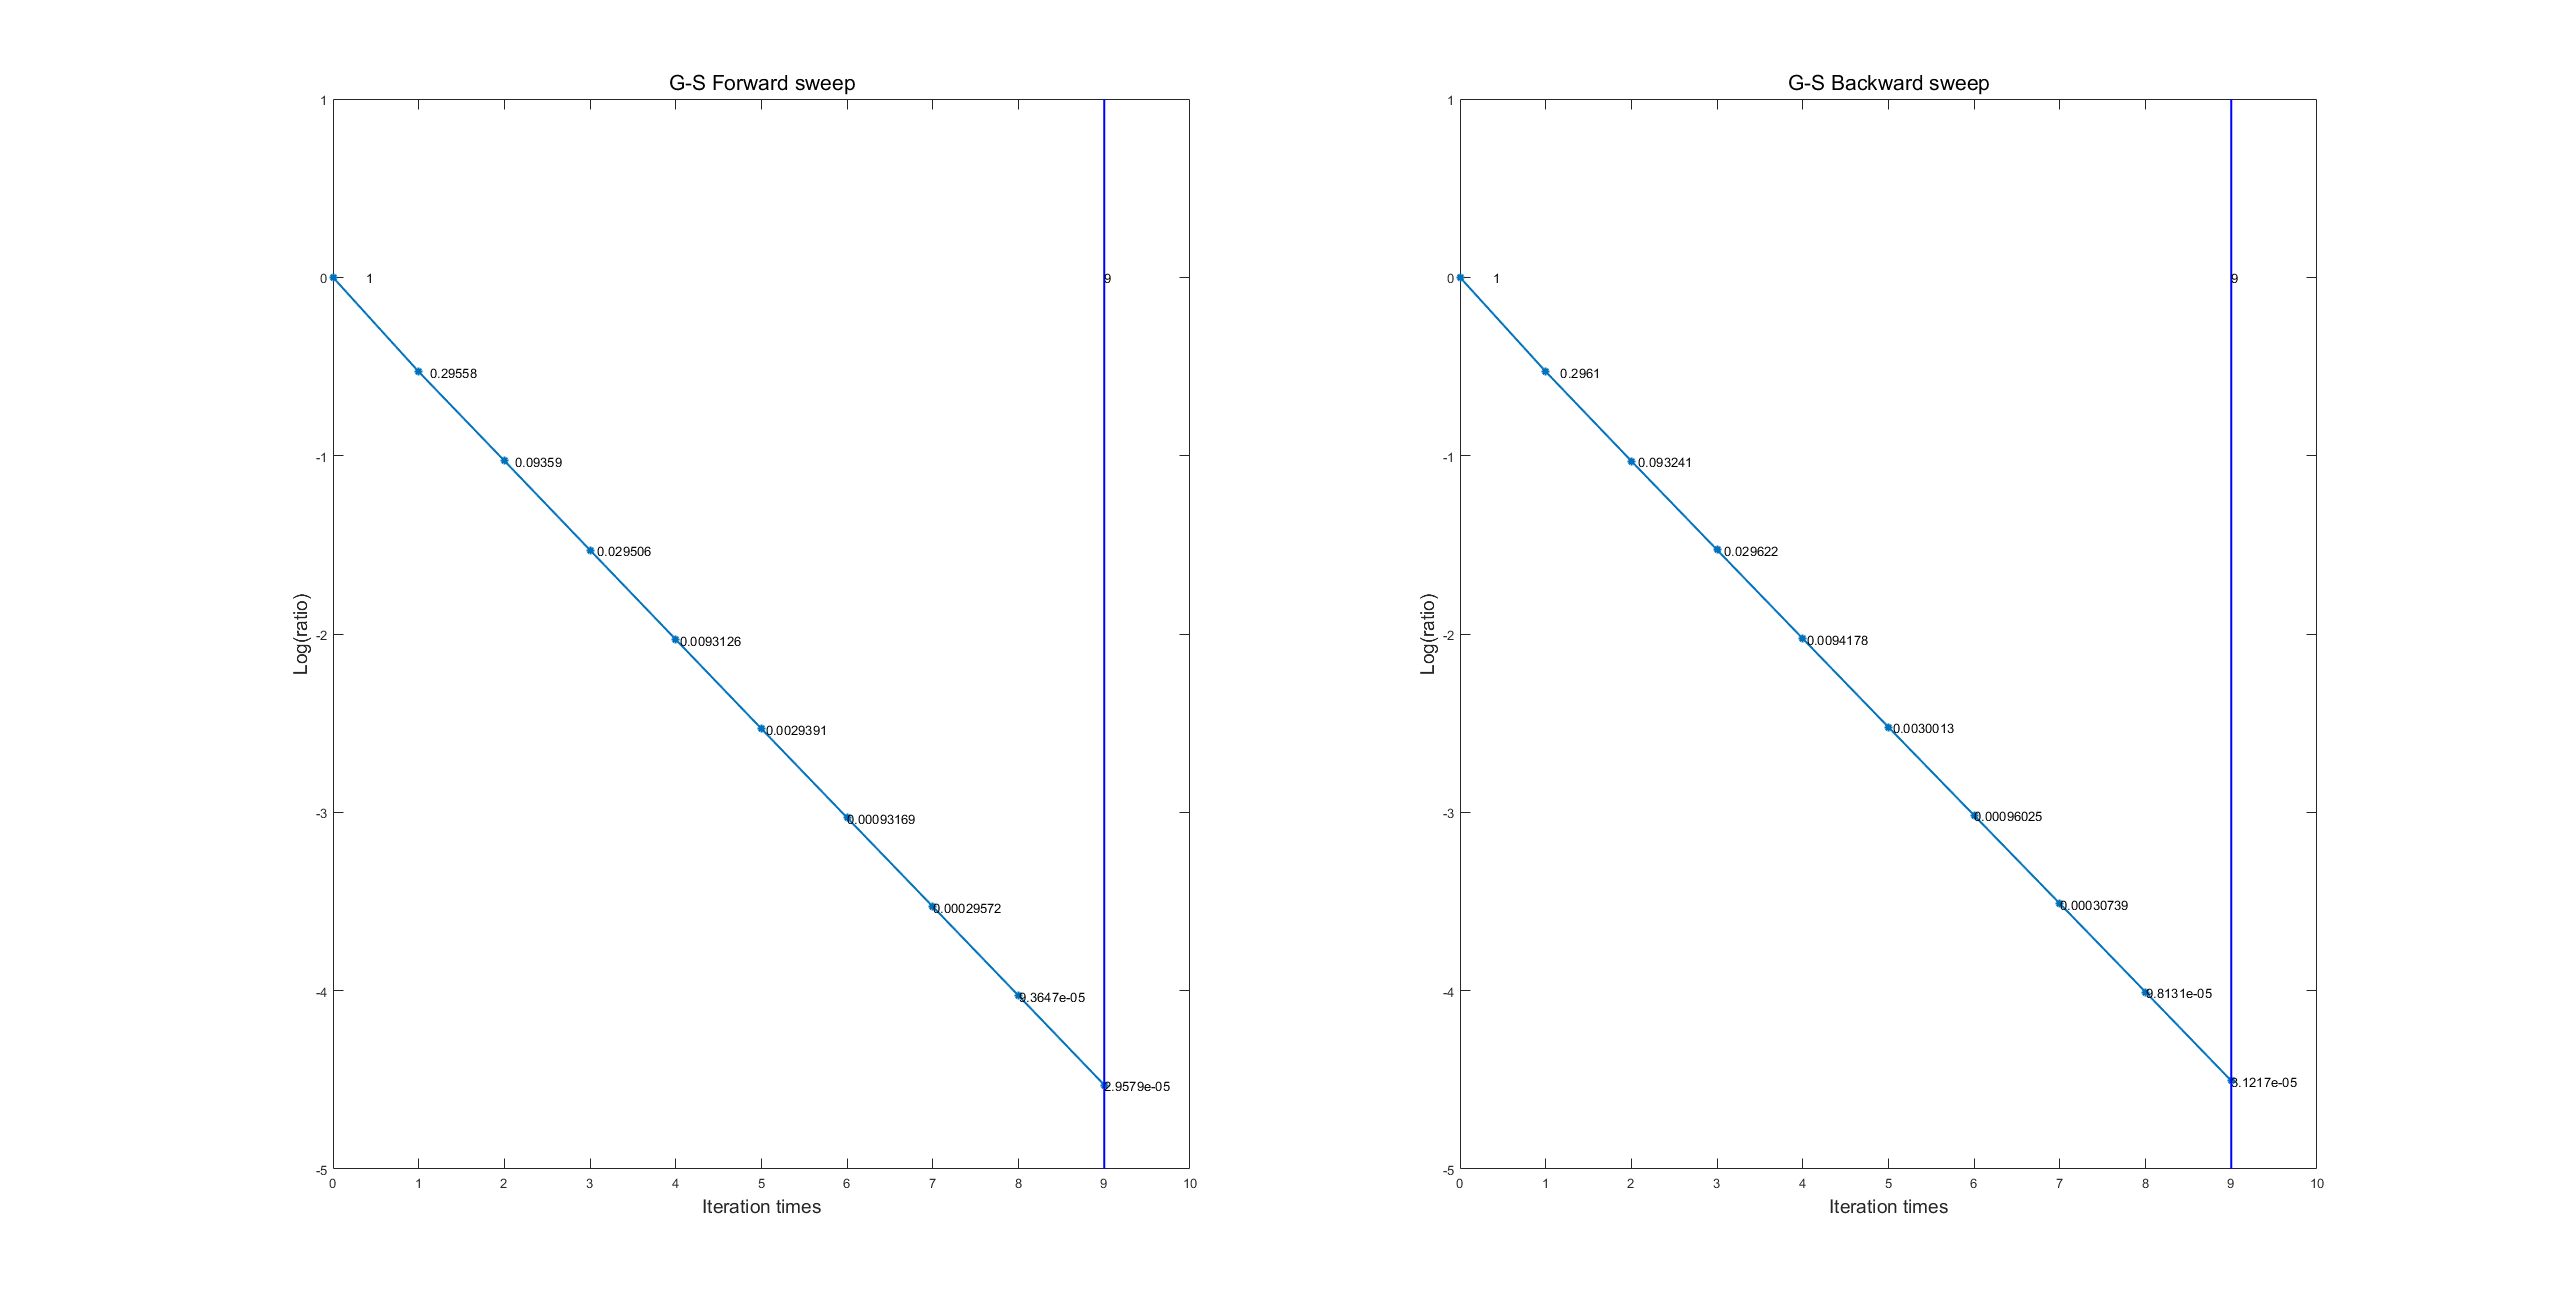
\includegraphics[width=2.5in]{G-S迭代-tol=10^(-5)rand1.png} 
		}
		\hfill
		\subfloat[random2]{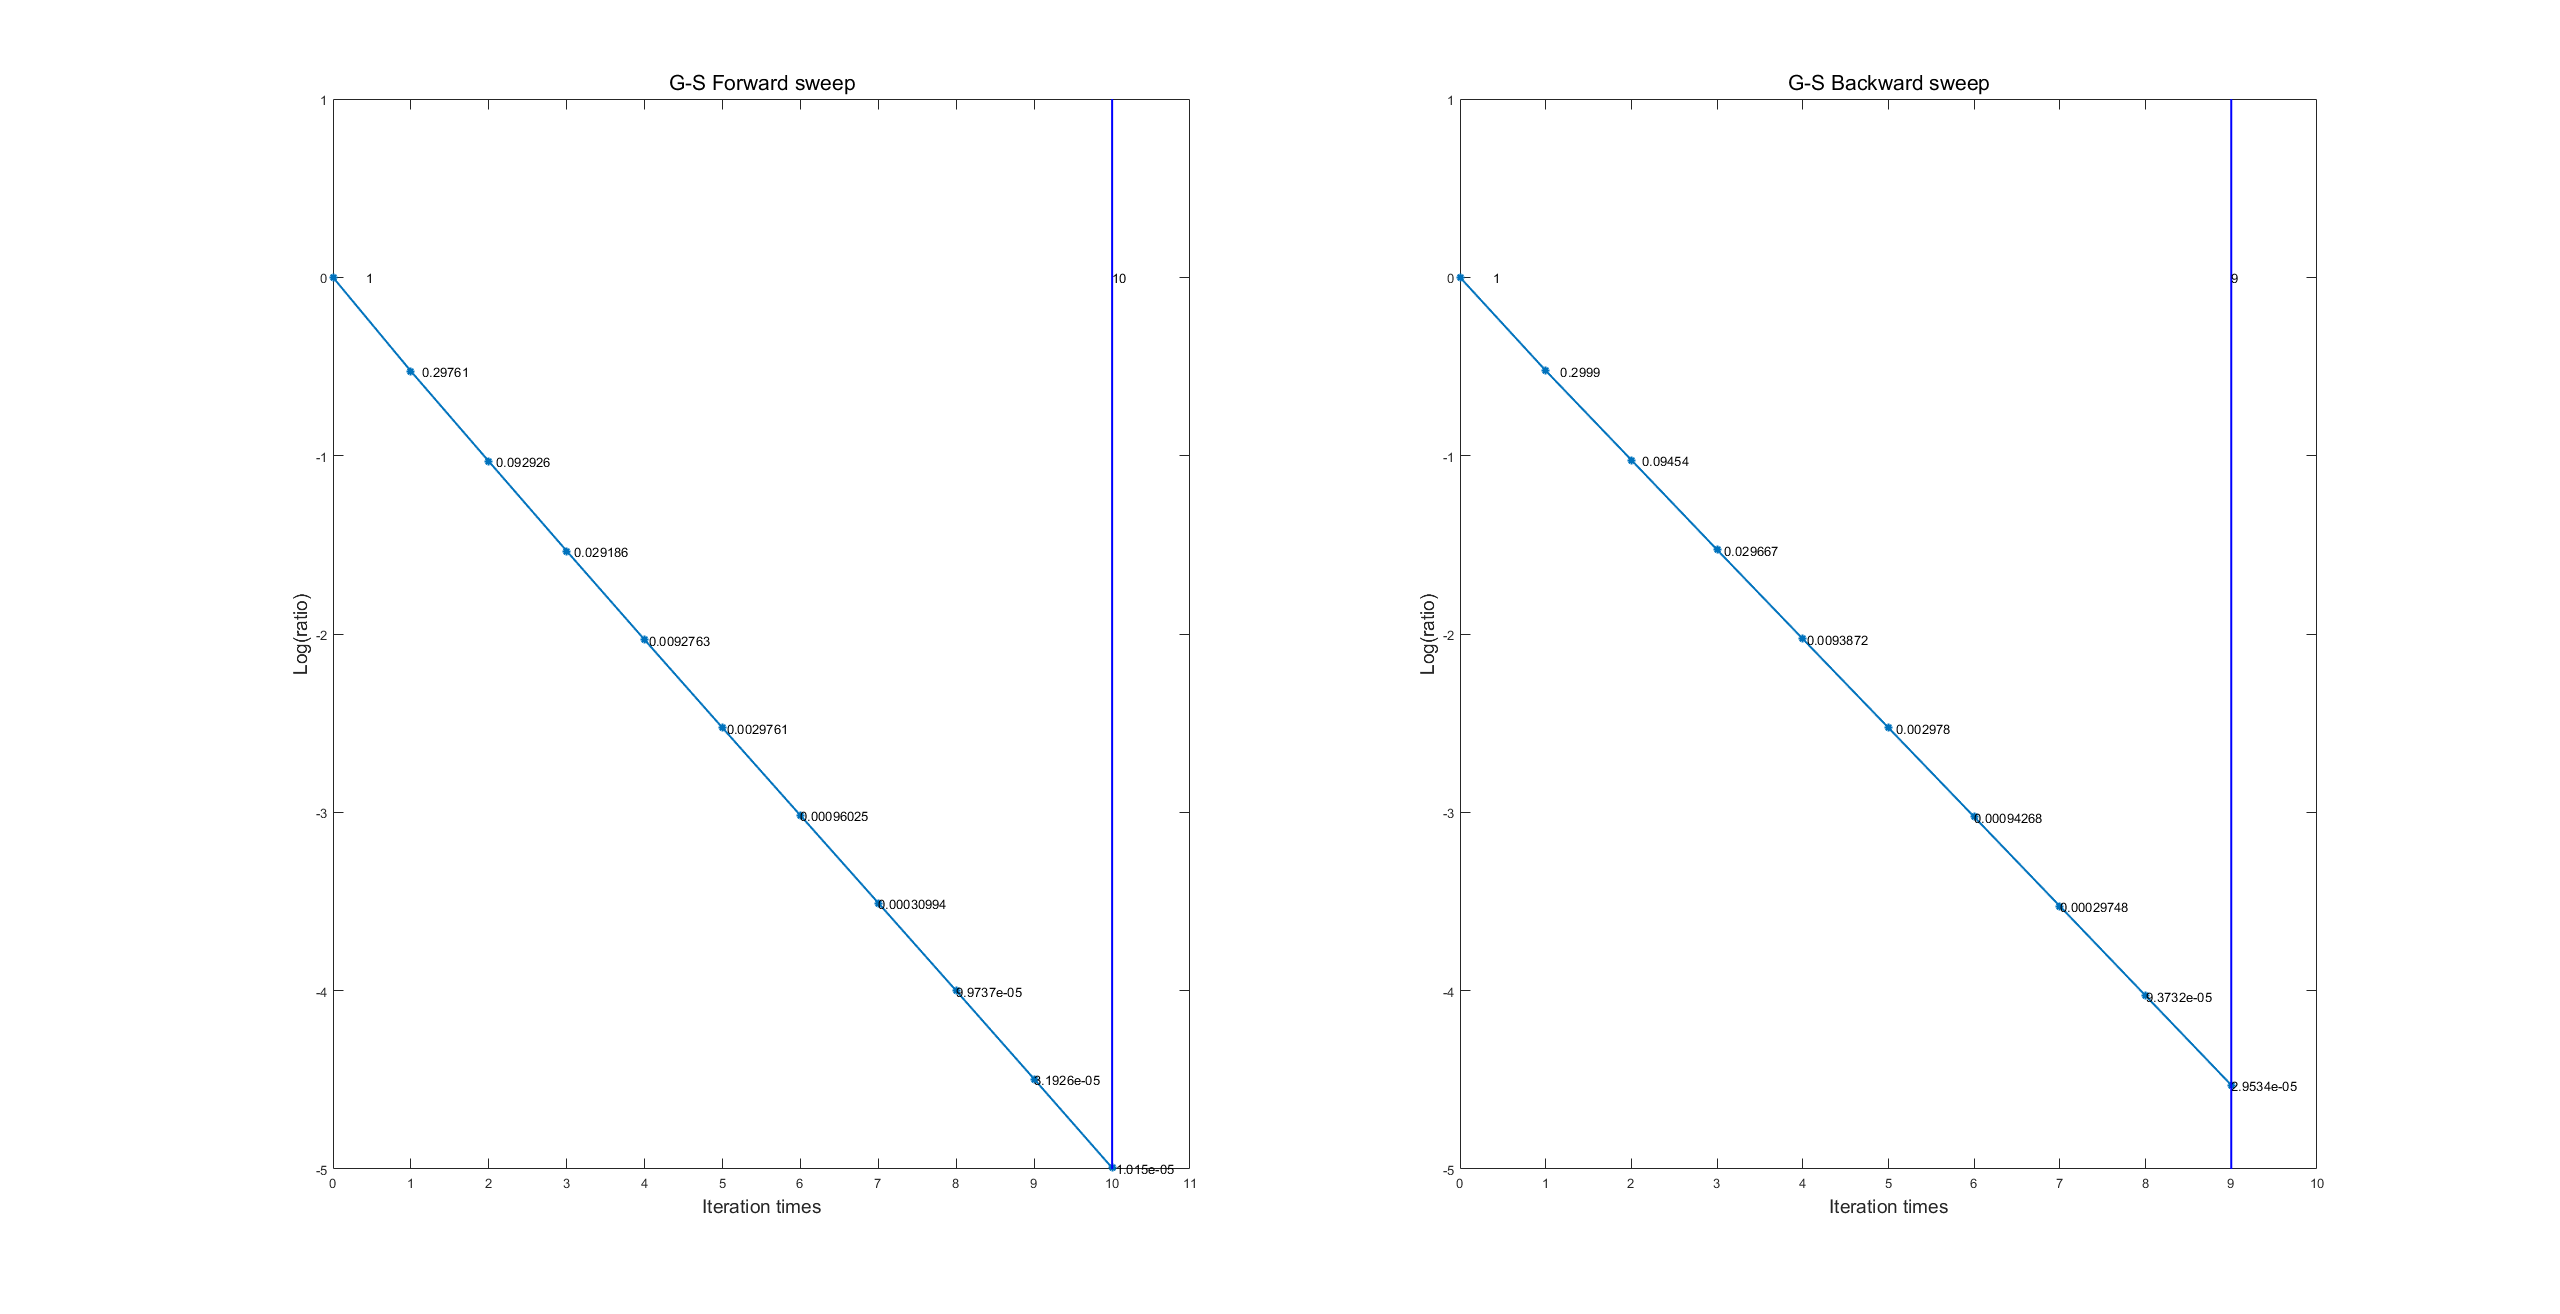
\includegraphics[width=2.5in]{G-S迭代-tol=10^(-5)rand2.png} }
		\newline
		\subfloat[random3]{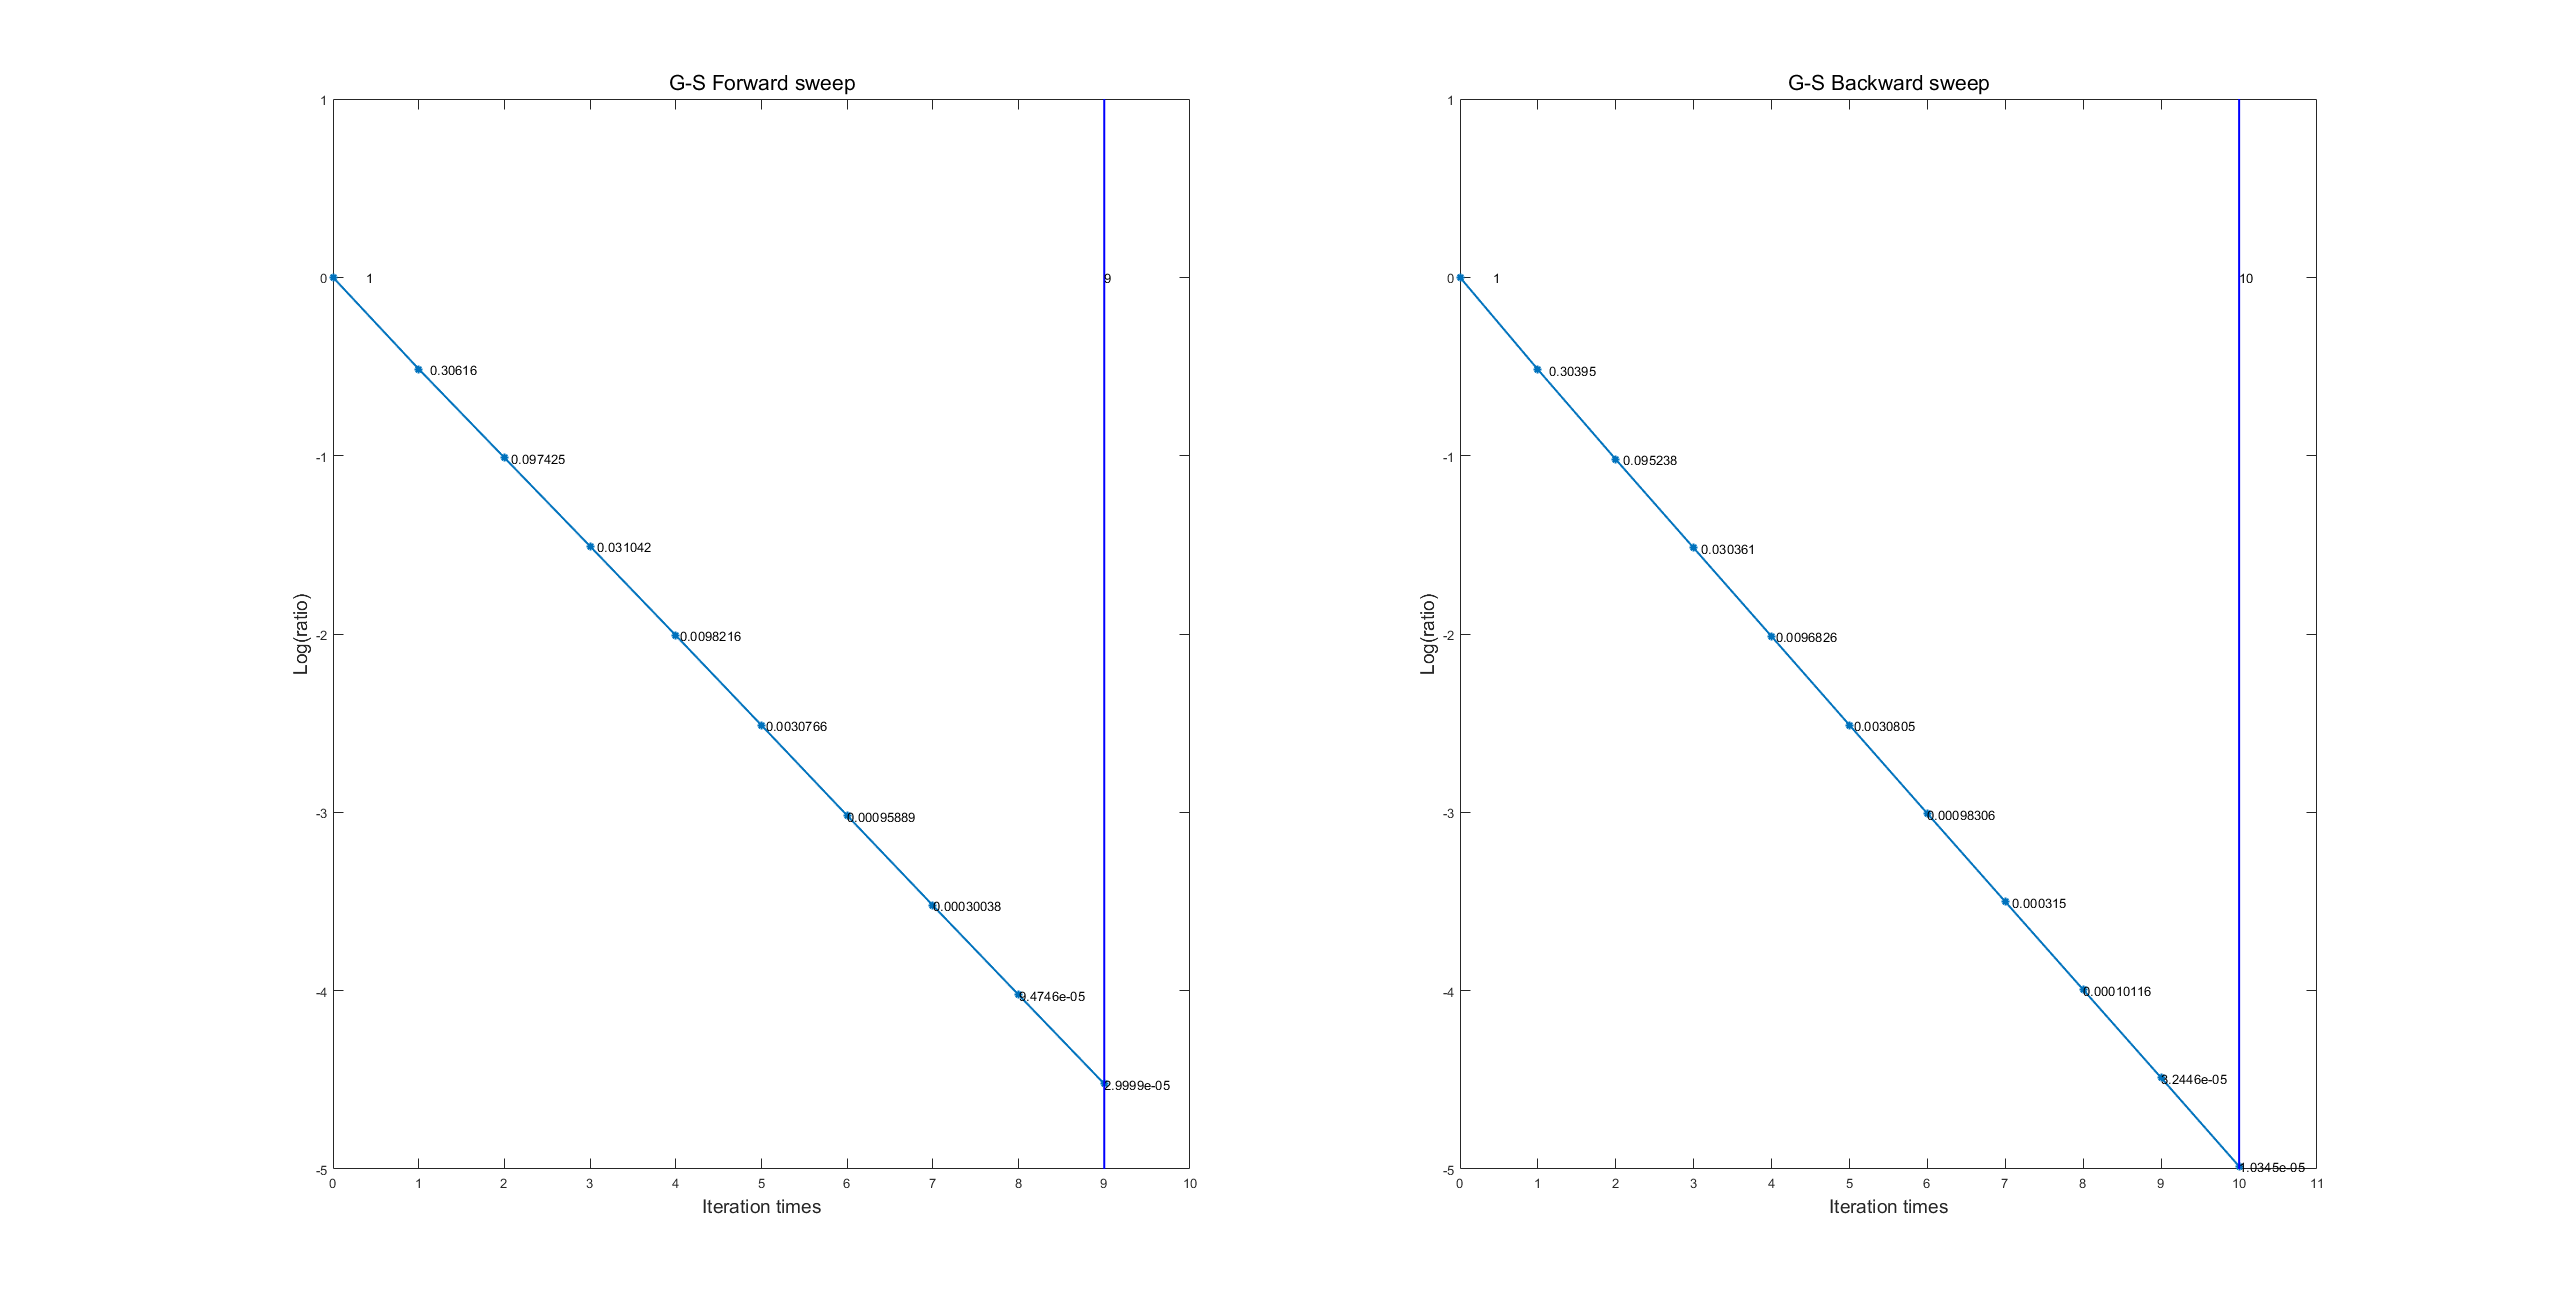
\includegraphics[width=2.5in]{G-S迭代-tol=10^(-5)rand3.png} }
		\hfill
		\subfloat[random4]{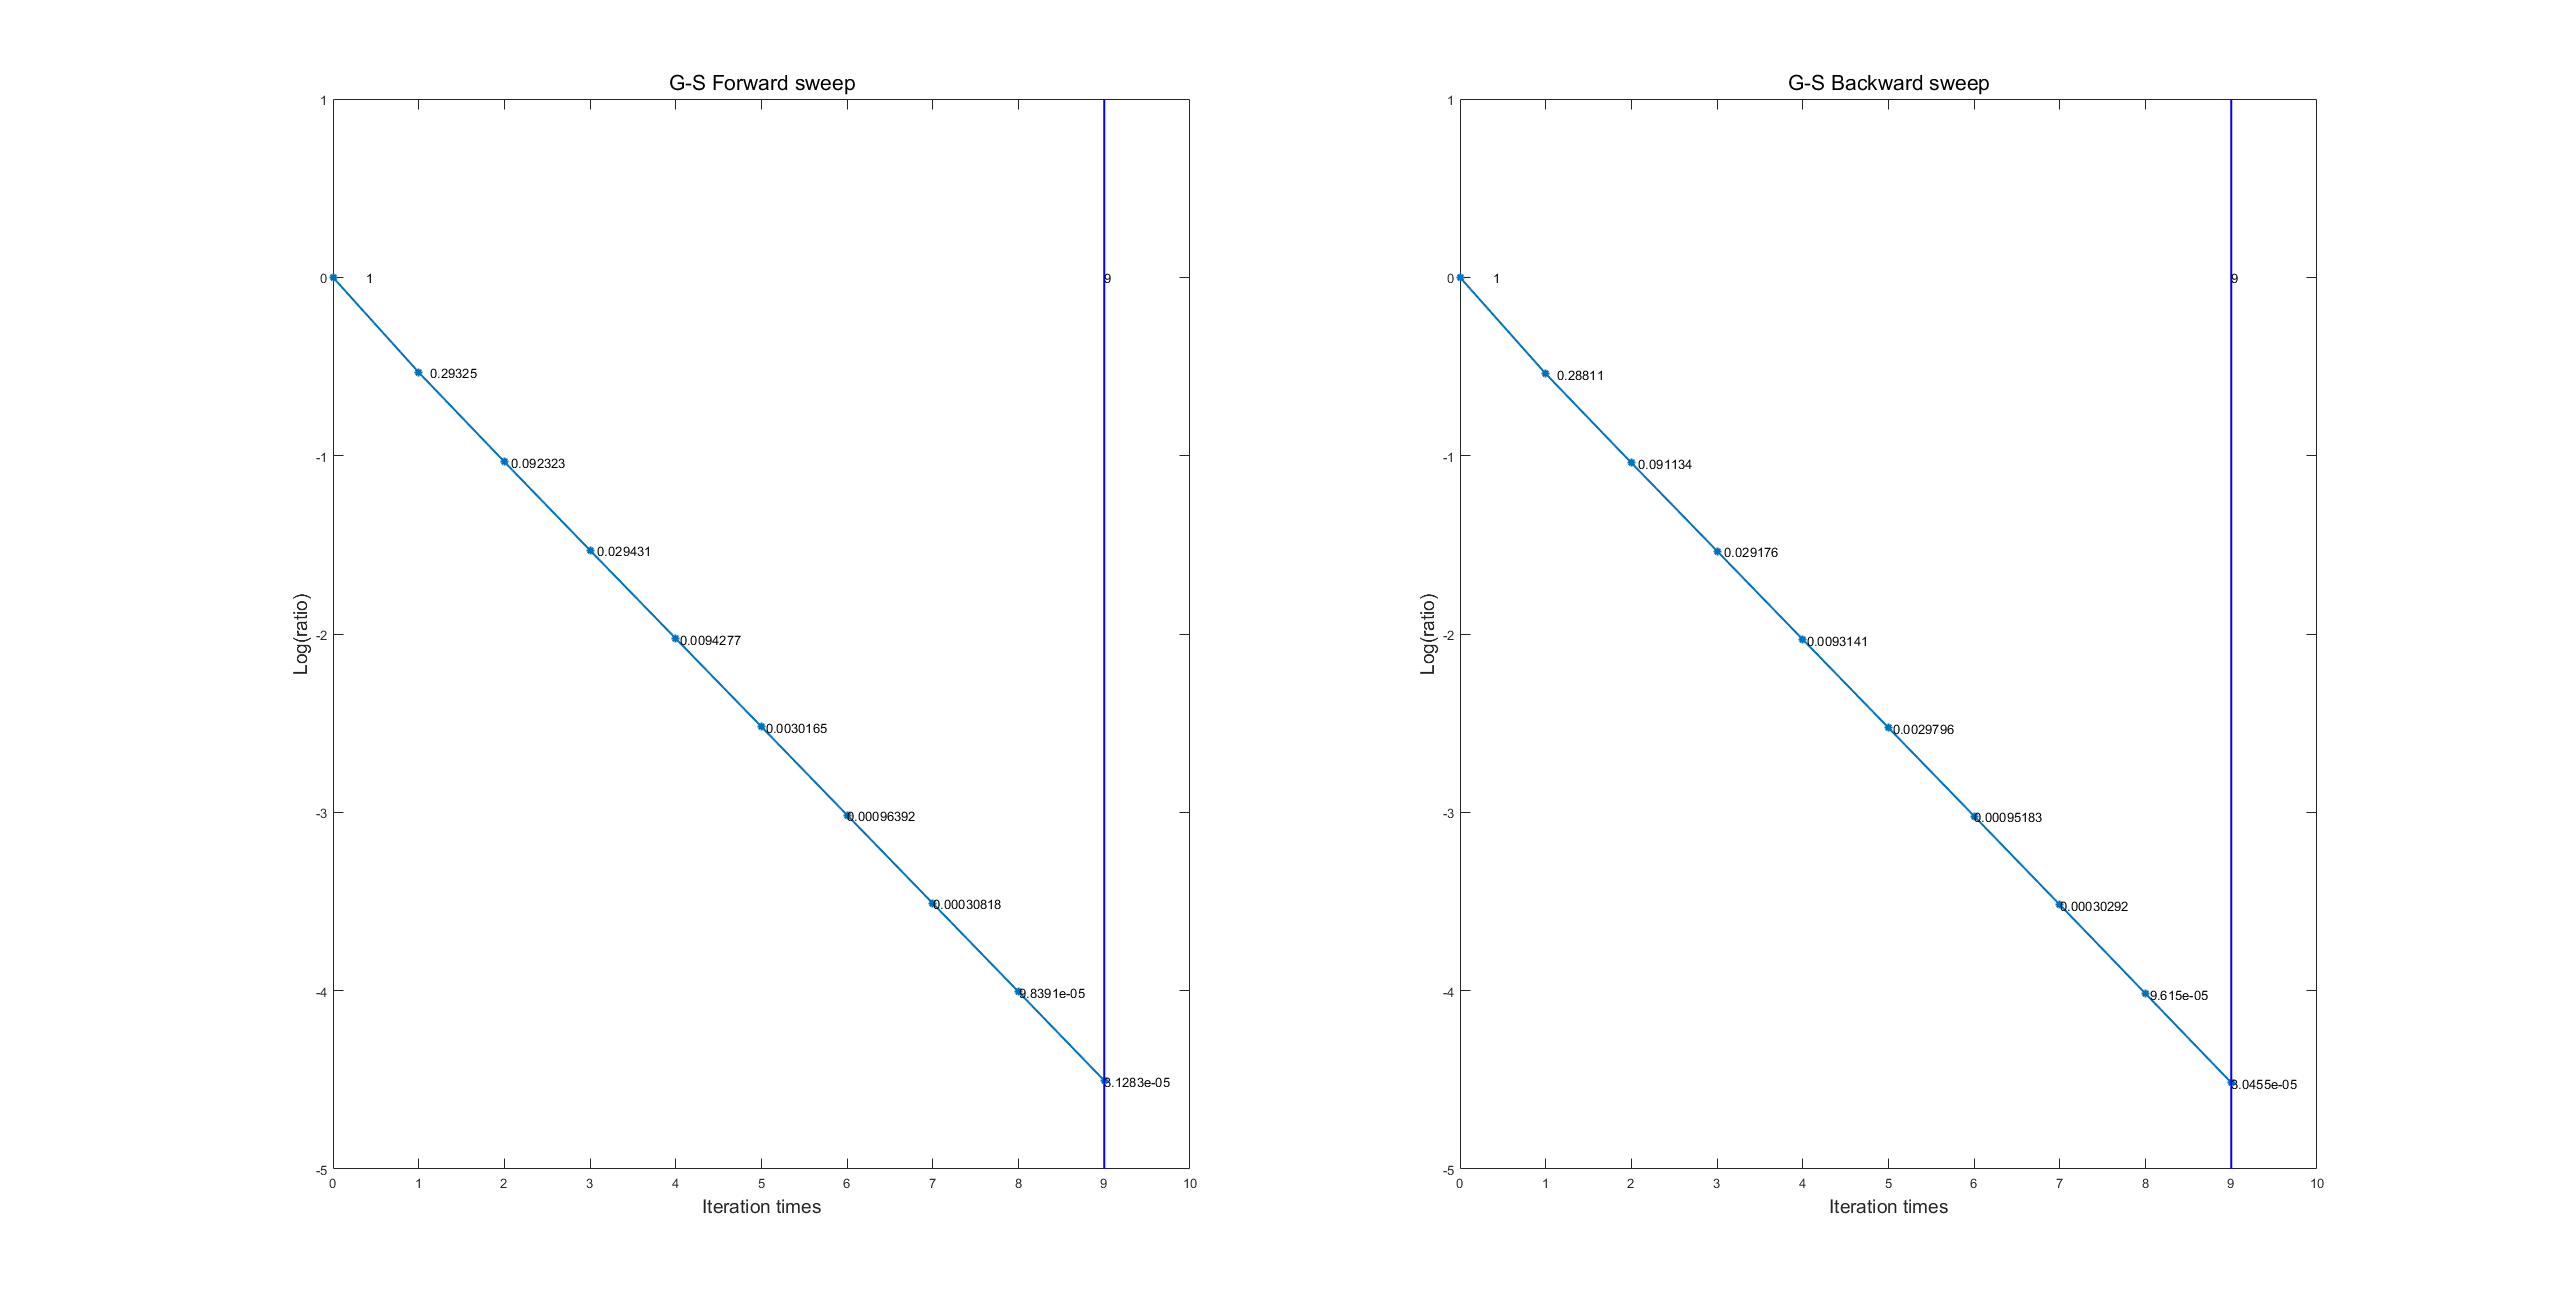
\includegraphics[width=2.5in]{G-S迭代-tol=10^(-5)rand4.png} }	
		\caption{高斯迭代次数和误差量级图}
	\end{figure}\\
\indent 观察图1可以看出,需要进行15次左右的雅克比迭代,方程的解才能小于迭代误差限制。观察图2可以看出,需要进行9次左右的高斯-赛德尔迭代,方程的解才能小于迭代误差限制。高斯-赛德尔迭代的收敛速度快于雅克比迭代。
	\vspace{10pt}\\
	\indent(2)取右端向量$b=\left[1,2,\cdots,20\right]^T$,初始向量$x^{\left(0\right)}=0$,将$A$的主对角线元素成倍增长,非主对角线元素不动,得到下图:\\
	\begin{figure}[!h]
		\centering
		\subfloat[element=3]{
			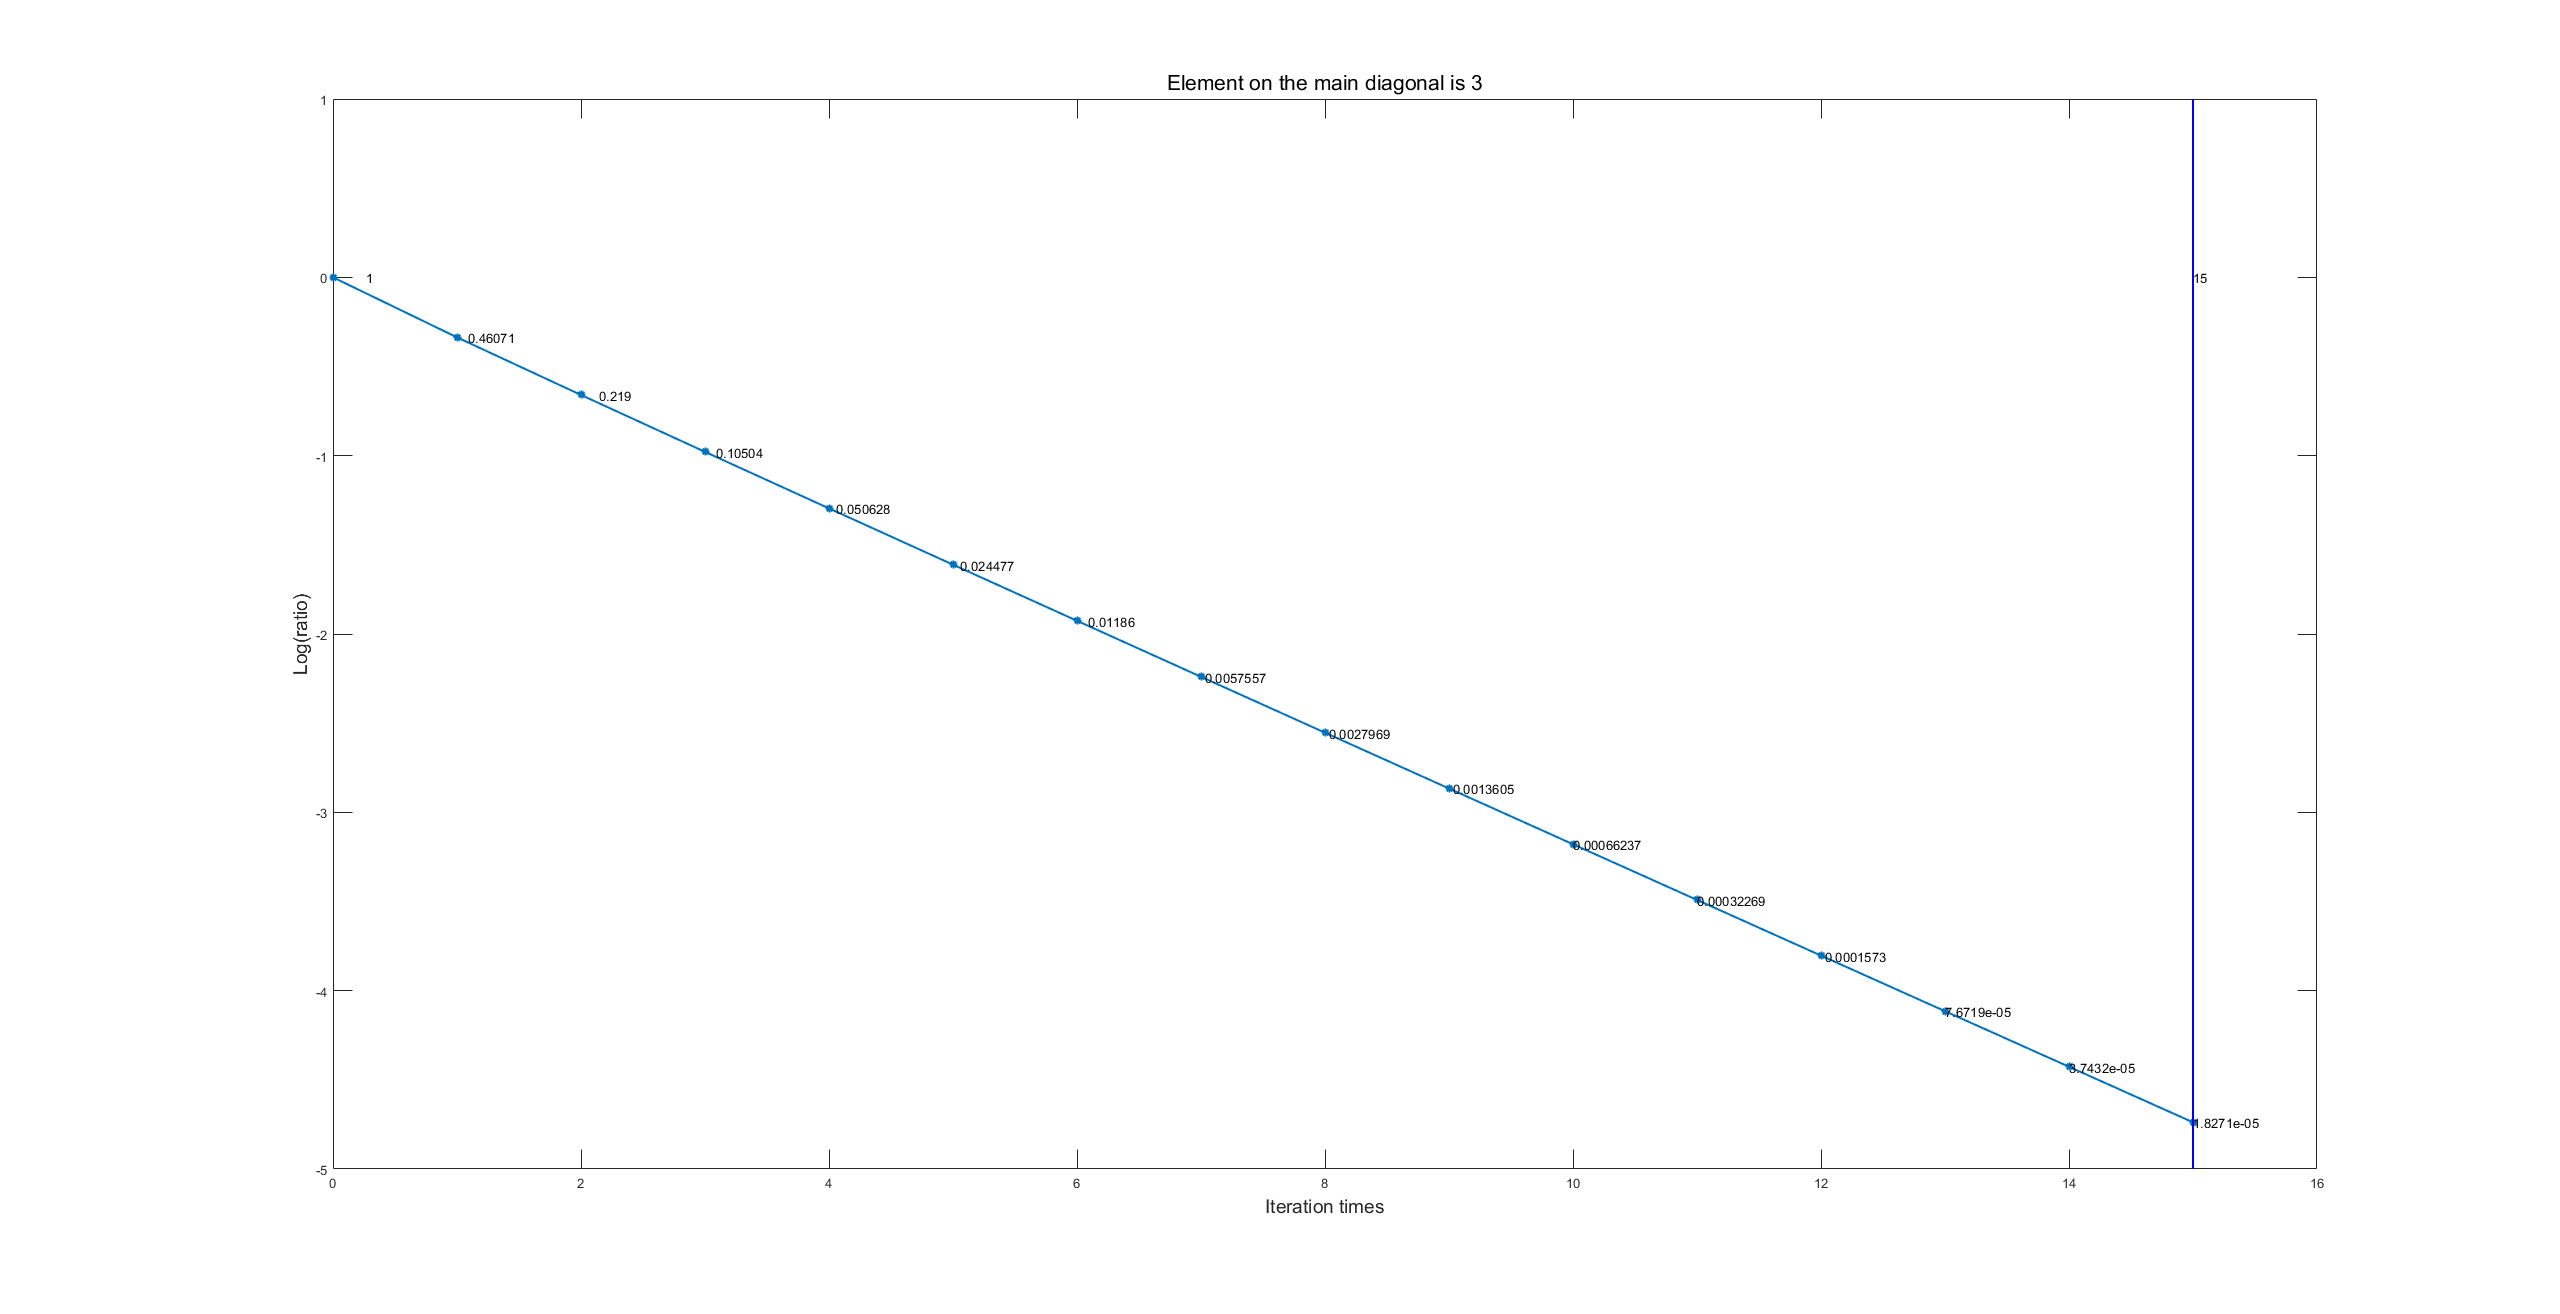
\includegraphics[width=3in]{element=3.png} 
		}
		\hfill
		\subfloat[element=6]{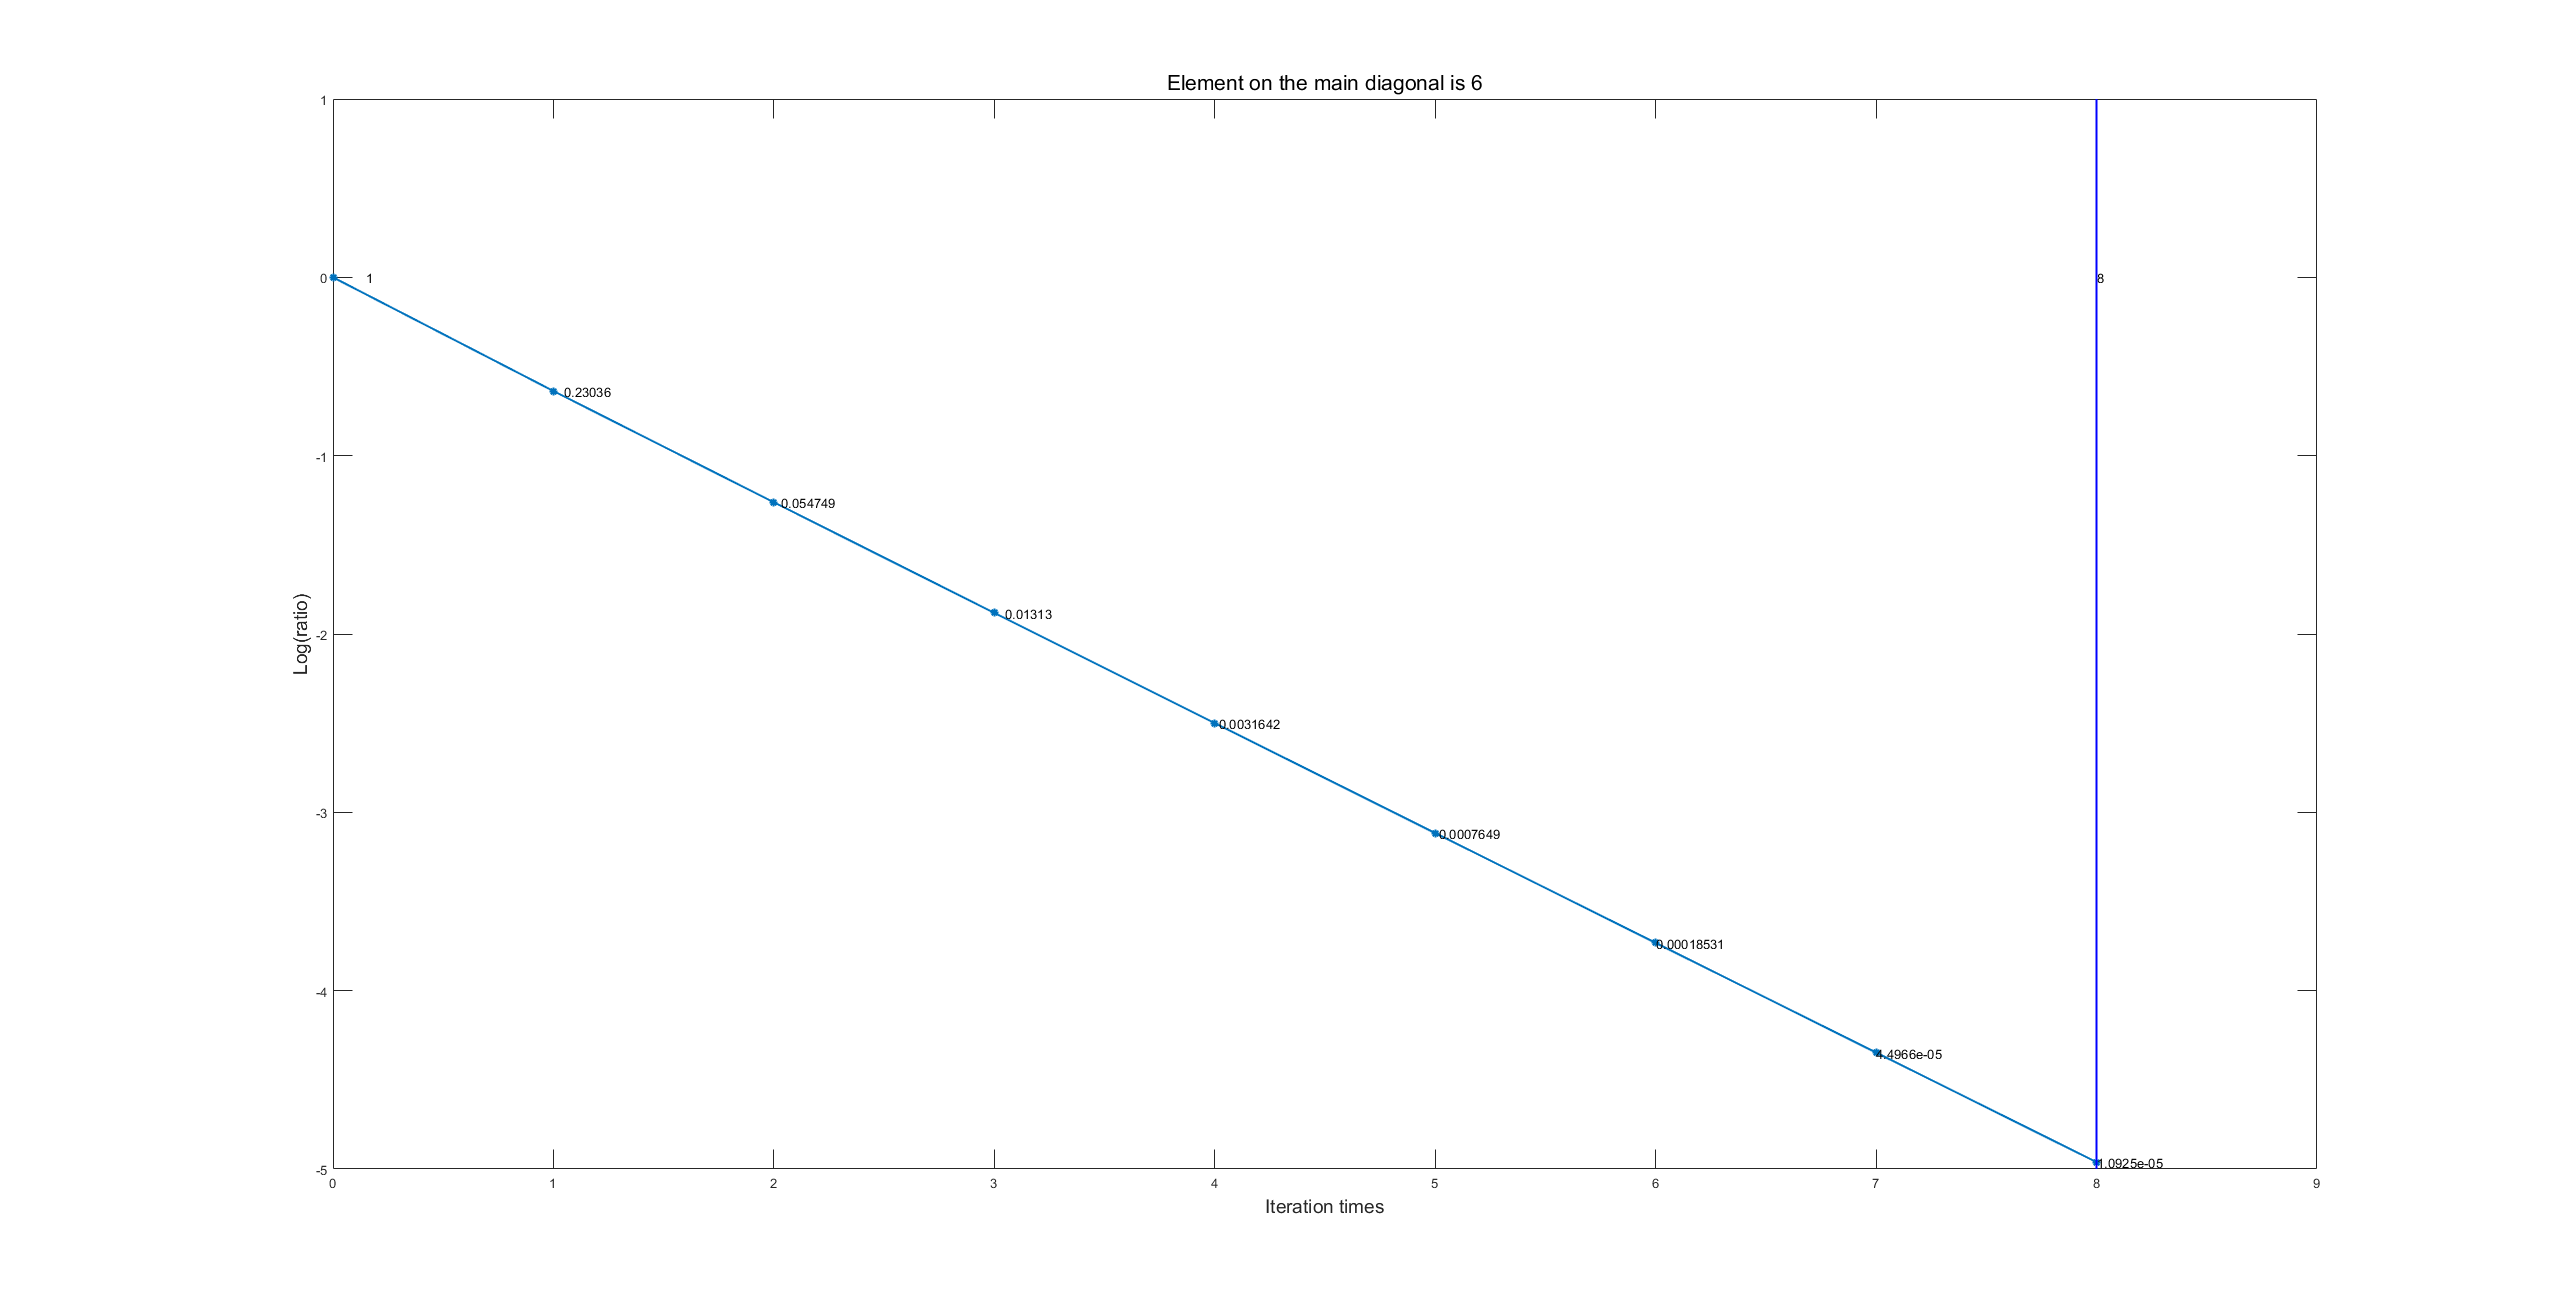
\includegraphics[width=3in]{element=6.png} }
		\newline
		\subfloat[element=12]{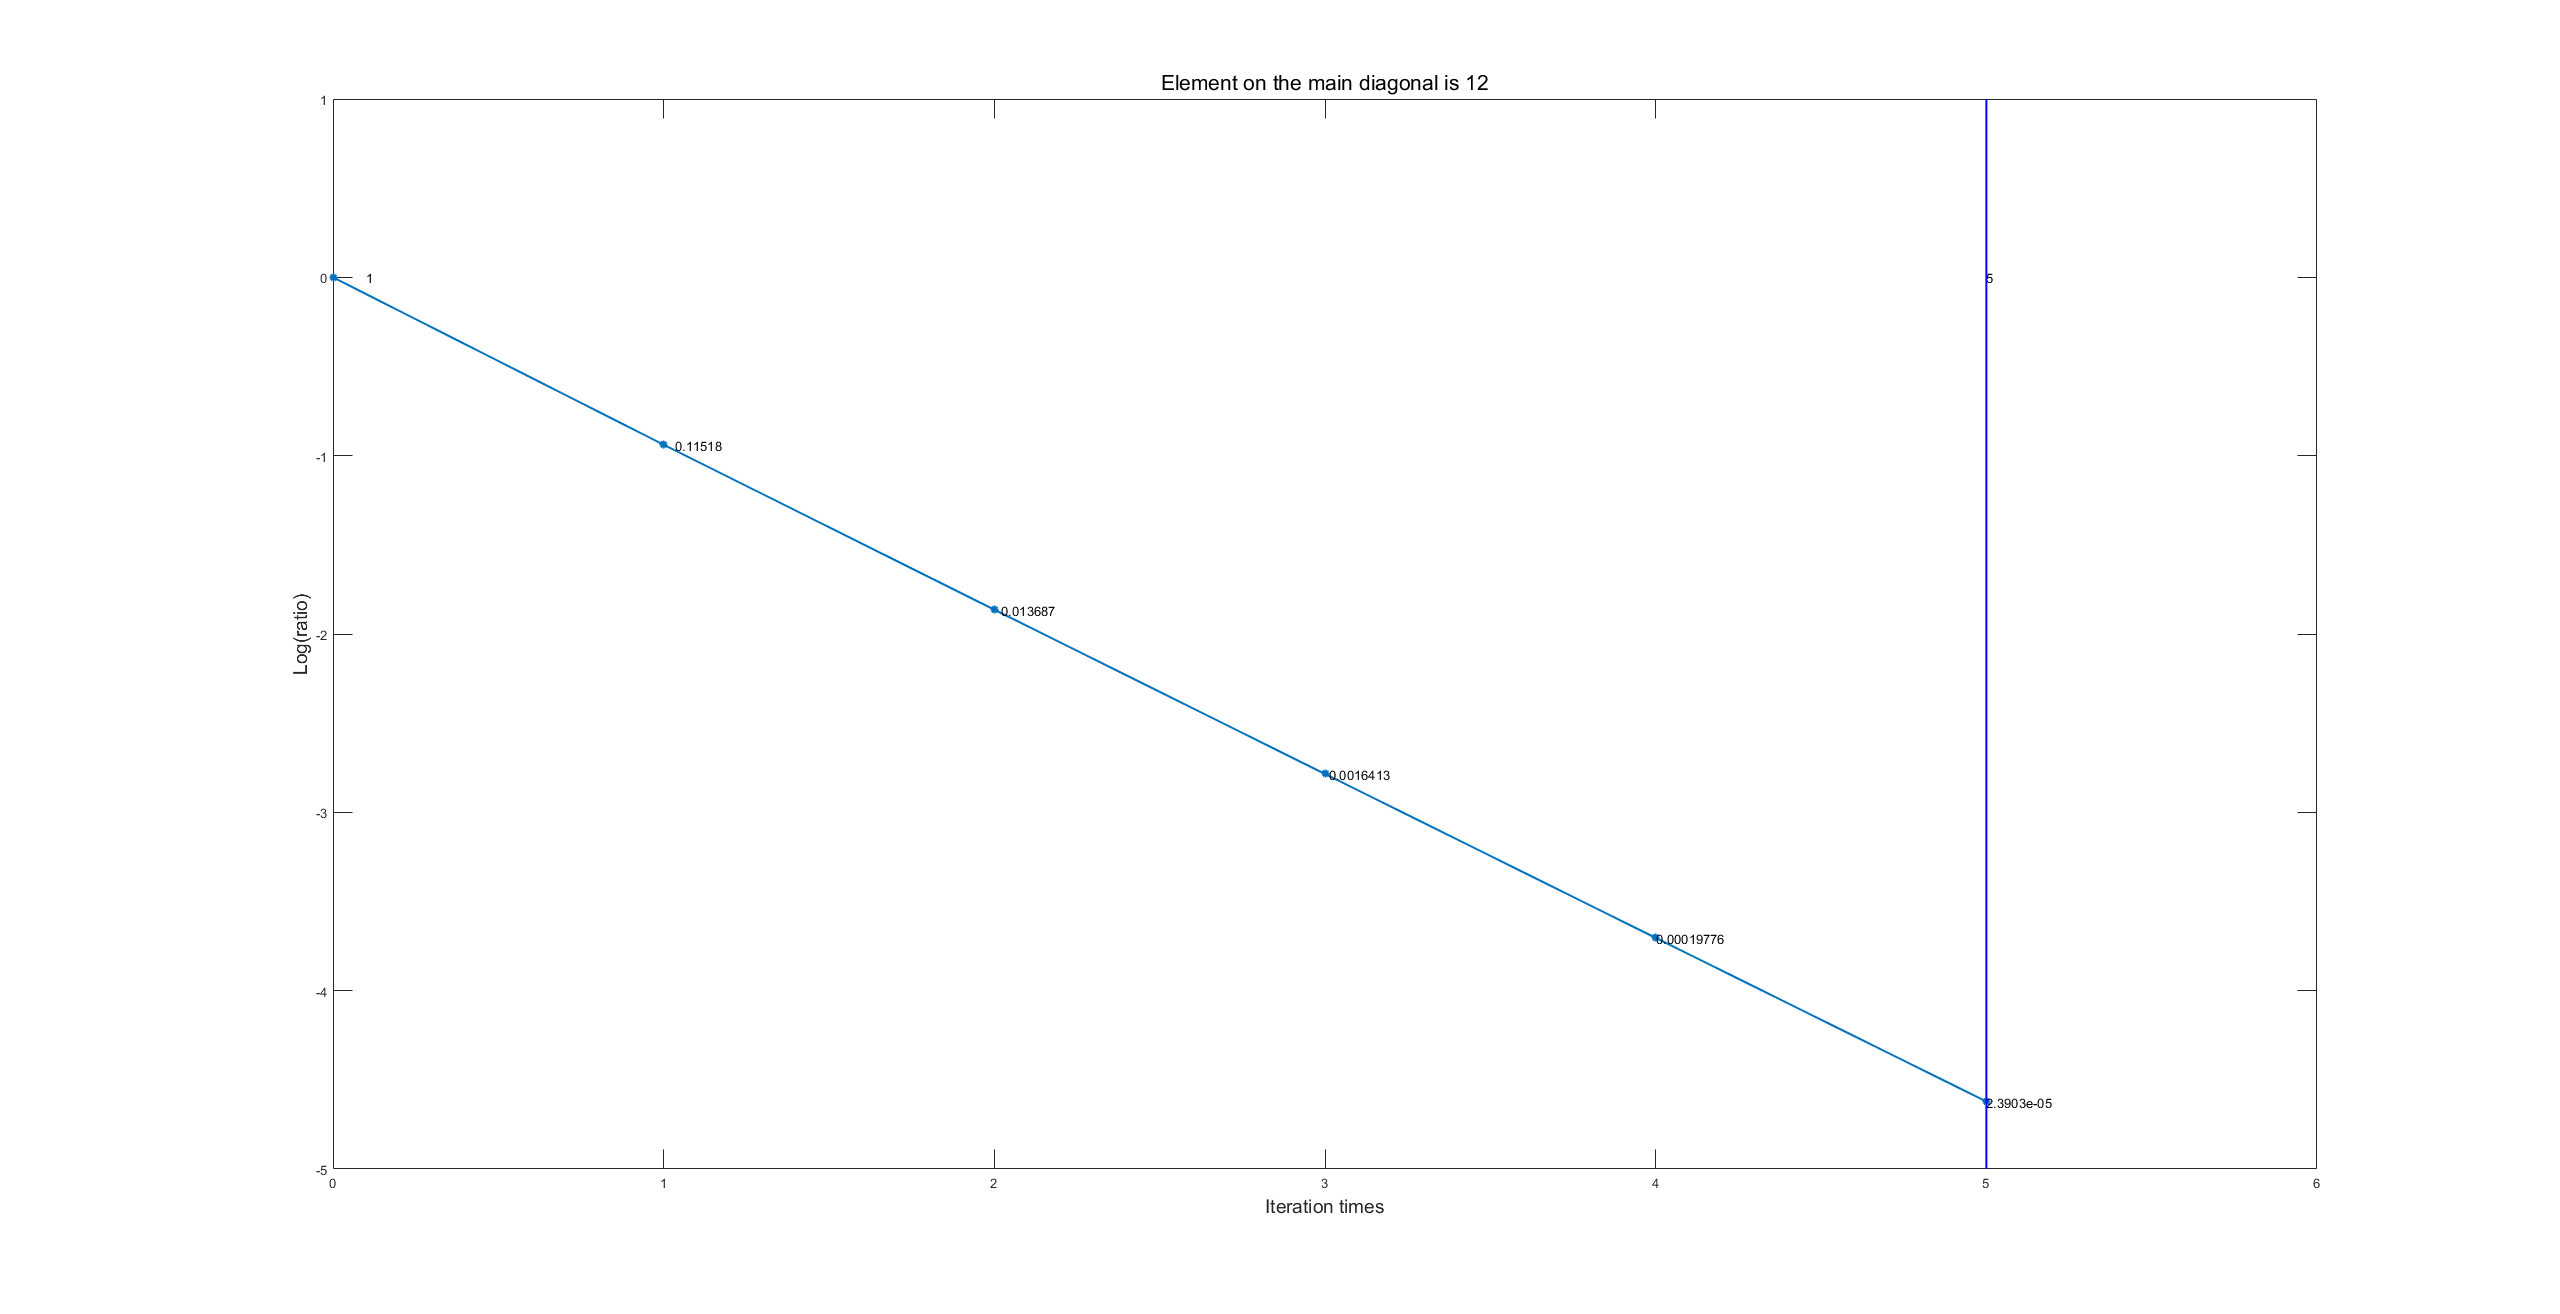
\includegraphics[width=3in]{element=12.png} }
		\hfill
		\subfloat[element=24]{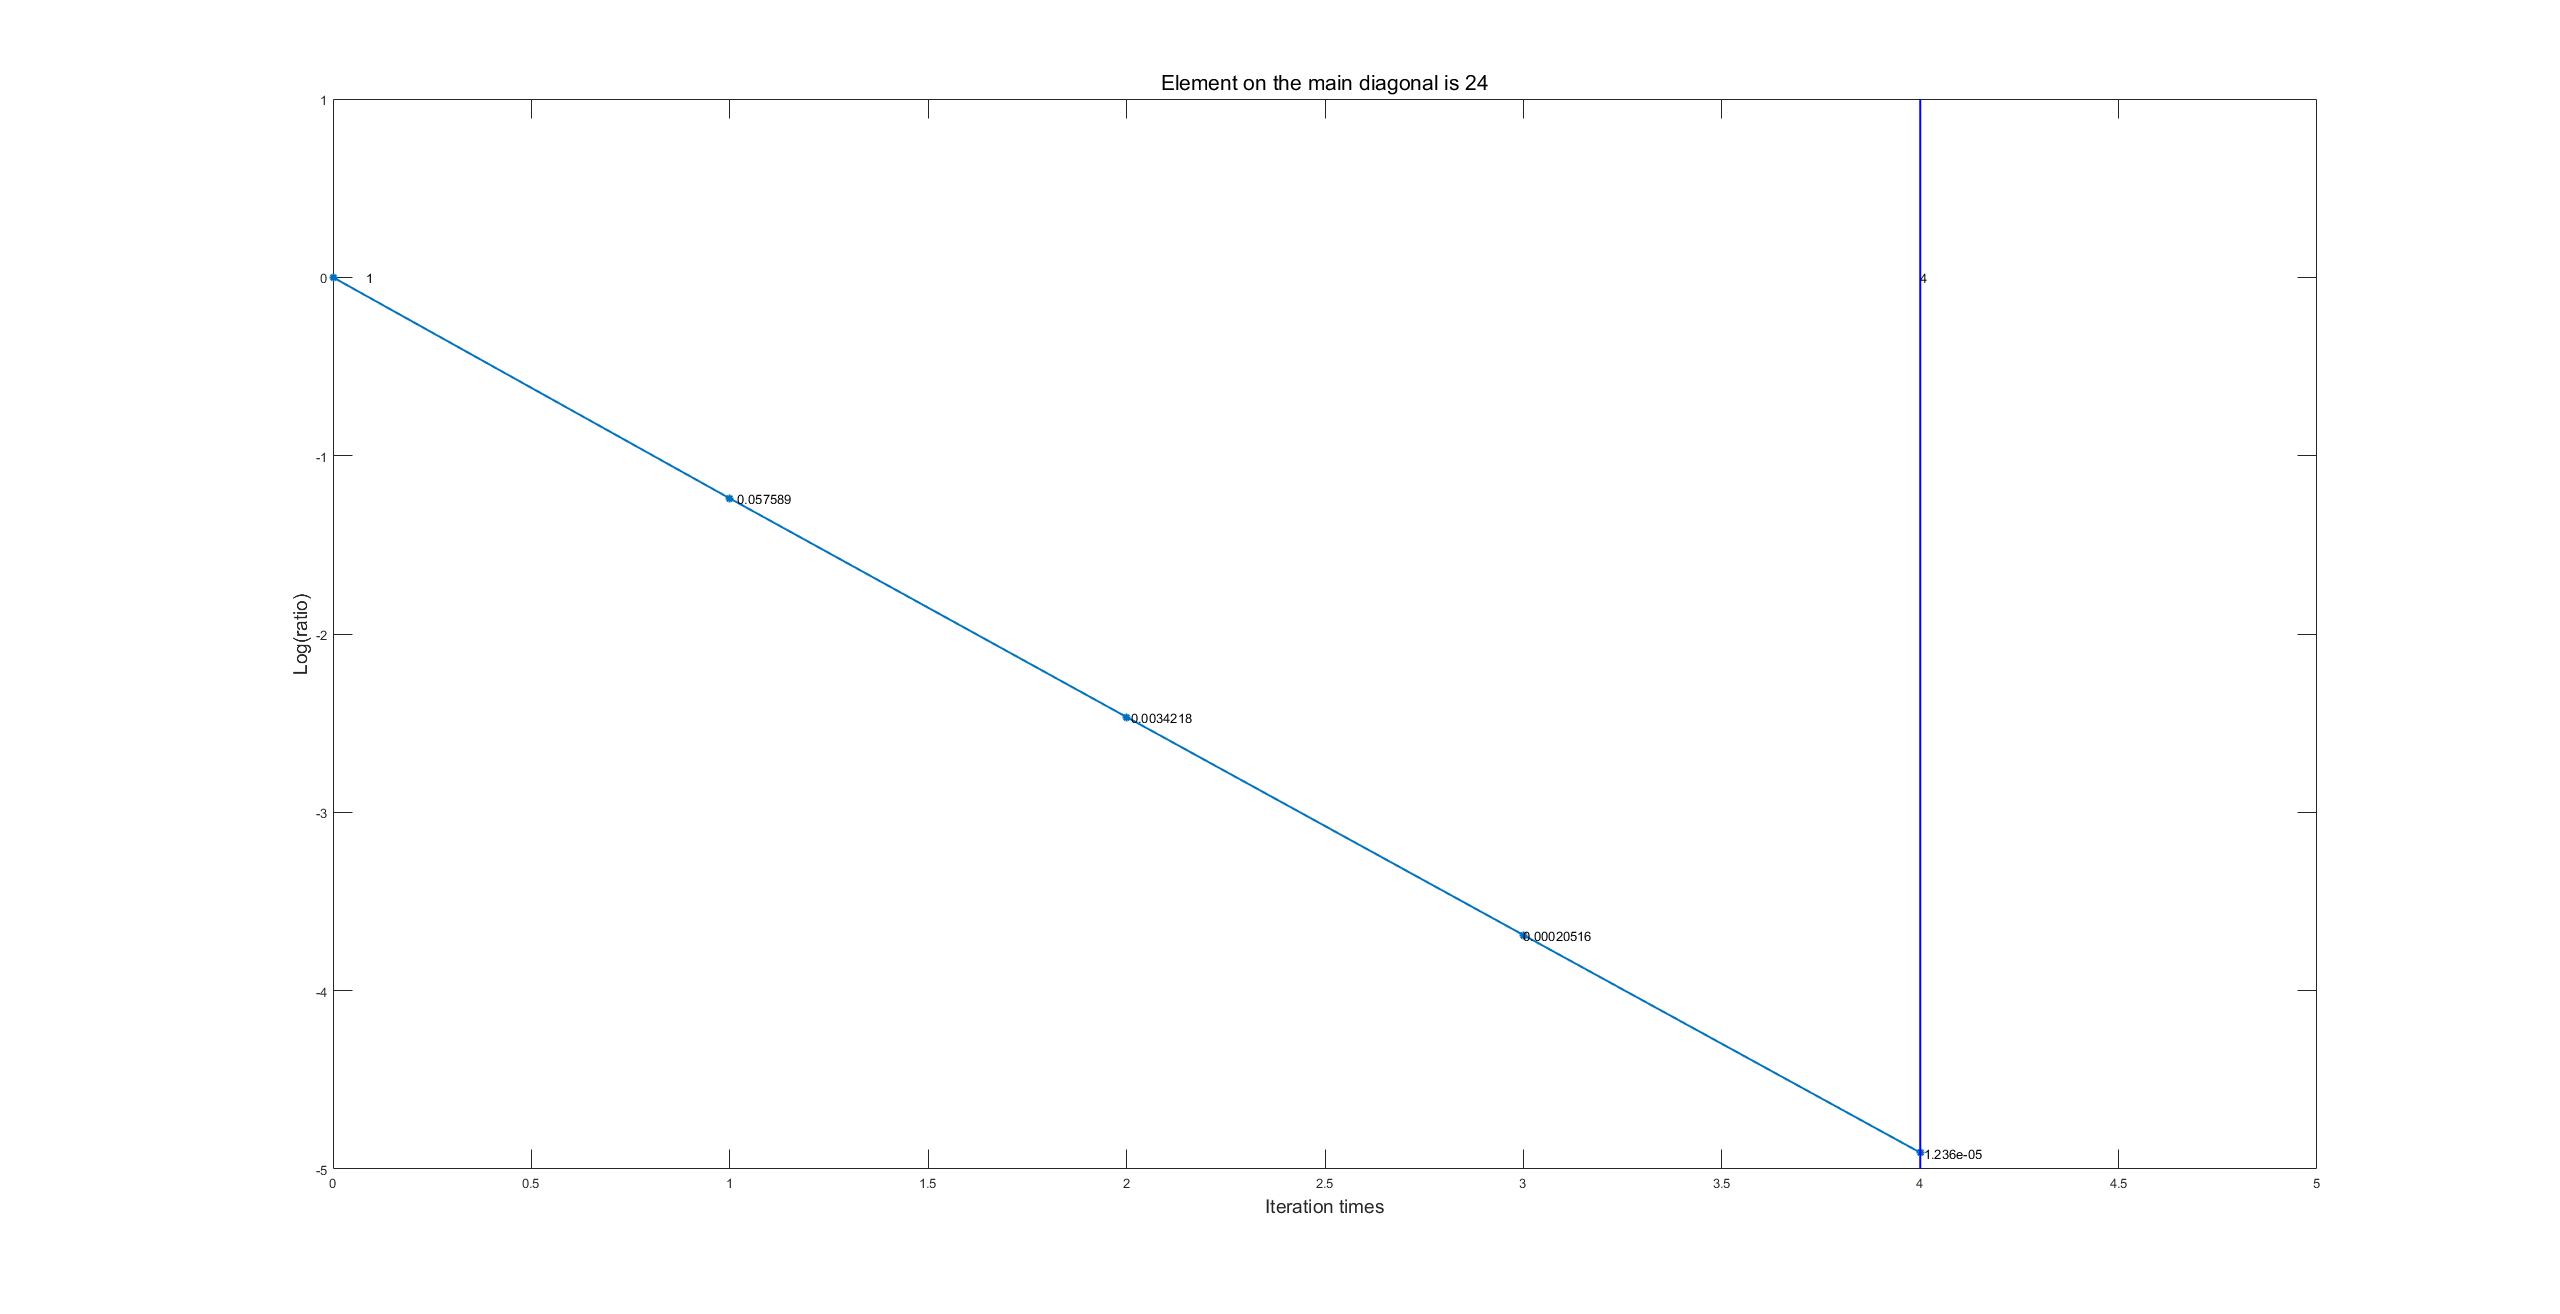
\includegraphics[width=3in]{element=24.png} }	
		\hfill
		\subfloat[element=48]{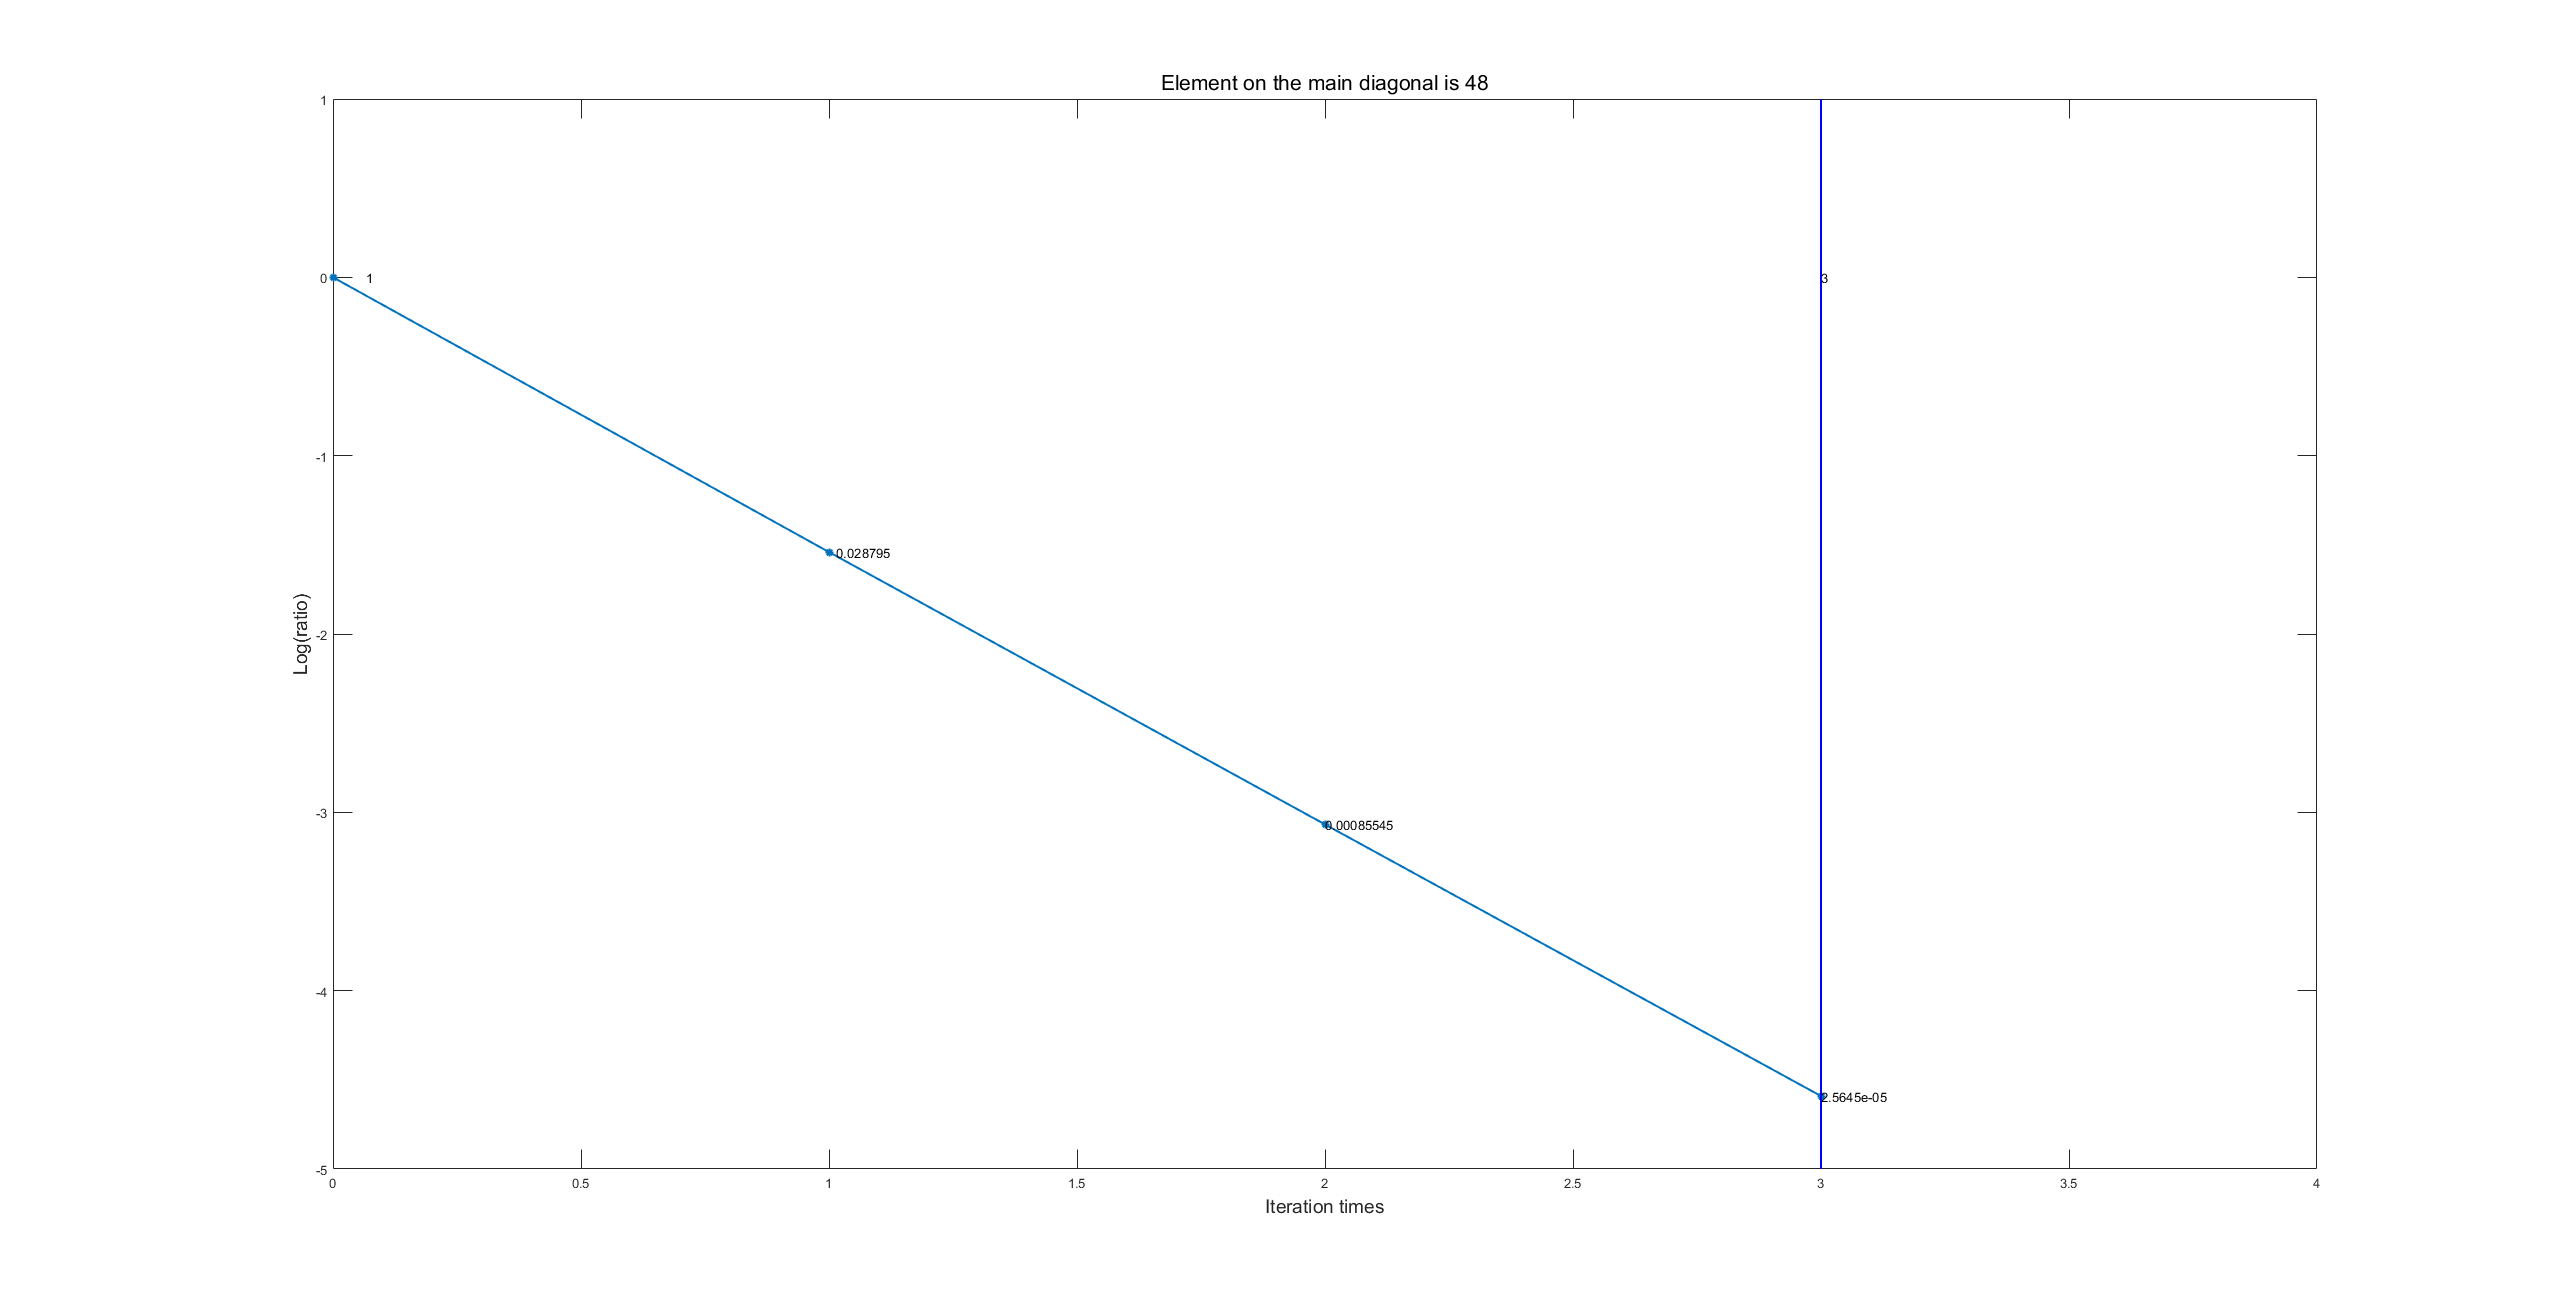
\includegraphics[width=3in]{element=48.png} }	
		\hfill
		\subfloat[element=96]{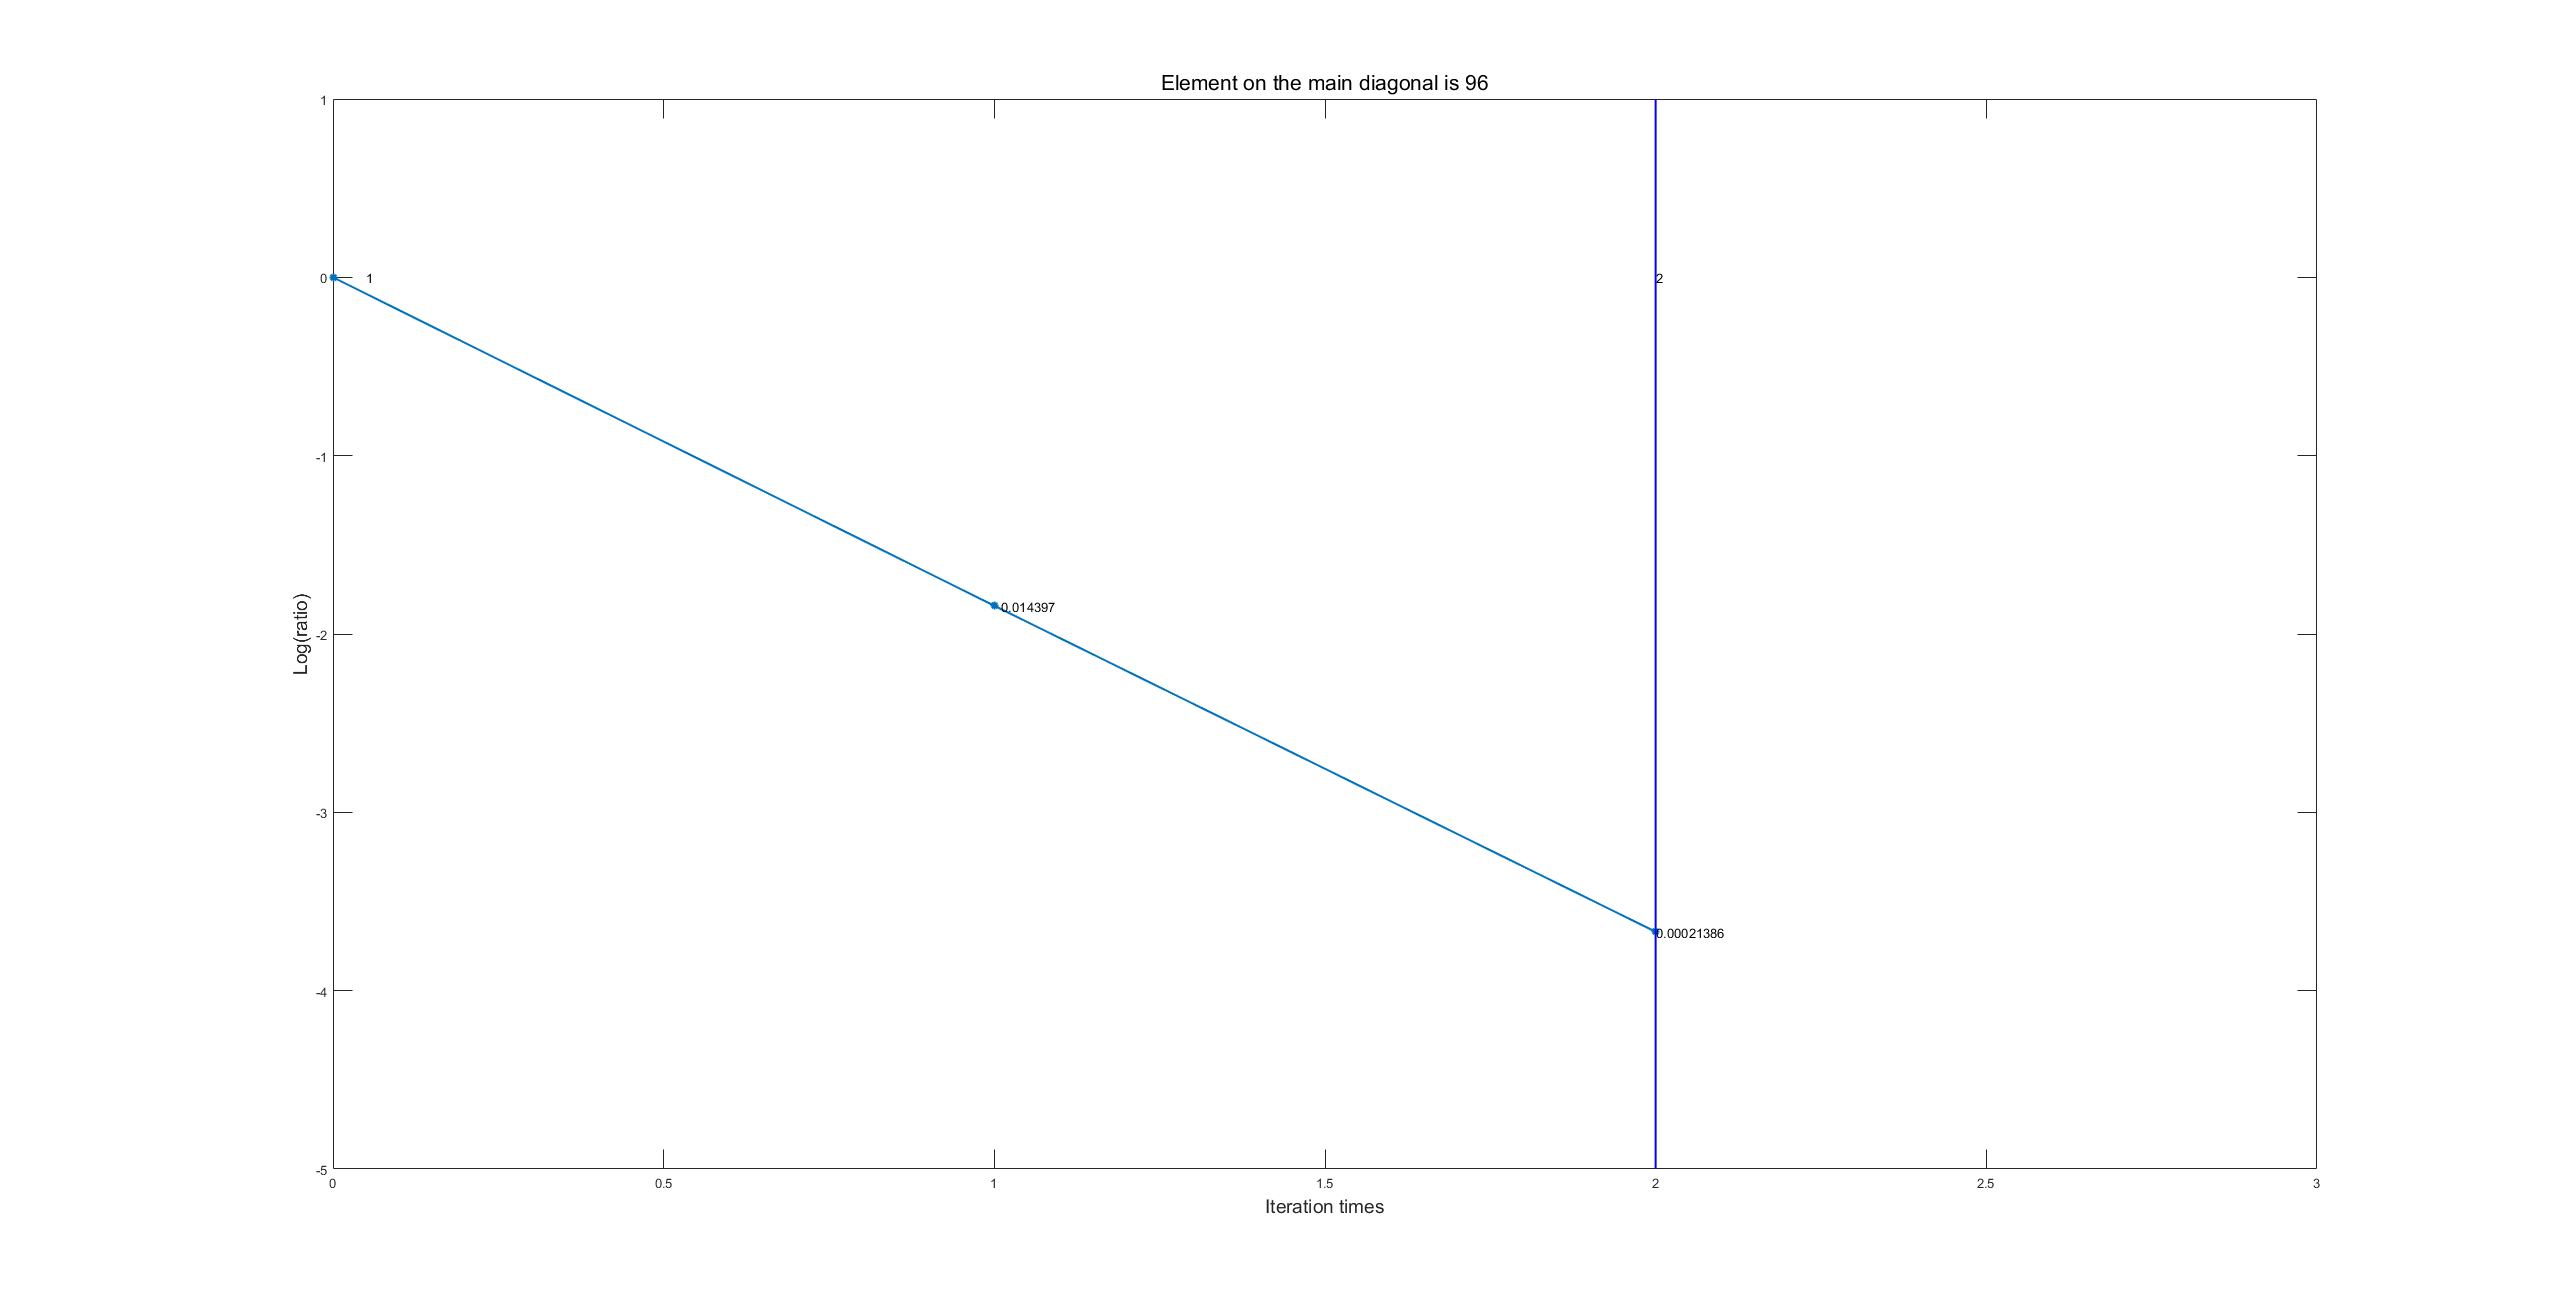
\includegraphics[width=3in]{element=96.png} }	
		\caption{主对角线元素与迭代次数图}
	\end{figure}\\
	\indent 观察图3,很明显主对角线元素越大,雅克比迭代次数约少。原因可能是随着主对角线元素的增大,矩阵$M$与$A$约接近,导致迭代次数减小。\\
	\newpage
	\indent(3)右端项和初始向量的取值与(2)	保持一致,给出不同$\omega$下G-S迭代与G-S(SOR)的对比图,以及S-G-S迭代与S-G-S(SOR)的对比图。\\
		\begin{figure}[!h]
		\centering
		\subfloat[G-S and G-S(SOR)]{
			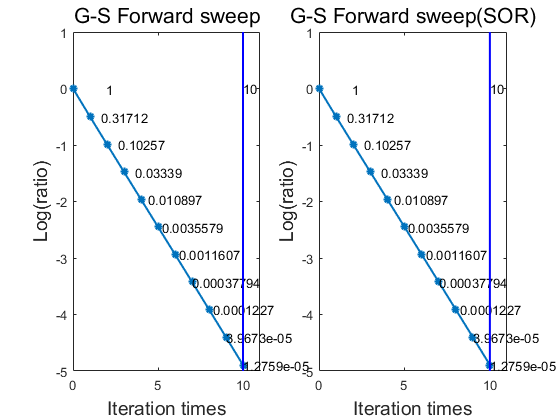
\includegraphics[width=3in]{gs与sorgs对比omega=1.png} 
		}
		\hfill
		\subfloat[S-G-S and S-G-S(SOR)]{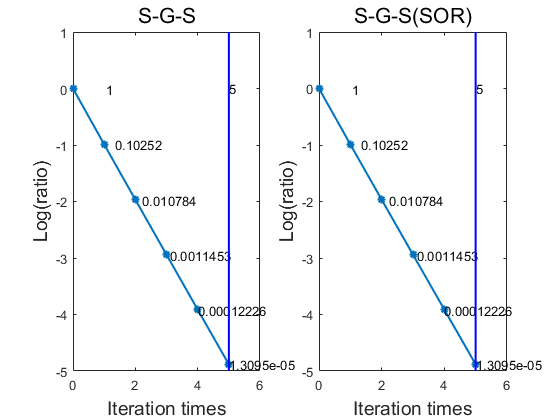
\includegraphics[width=3in]{sgs与sorsgs对比omega=1.png} }
		\caption{$\omega=1$对比}
	\end{figure}\\
	
	\begin{figure}[!h]
		\centering
		\subfloat[G-S and G-S(SOR)]{
			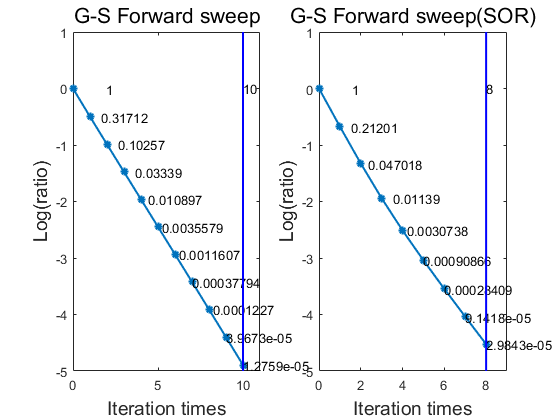
\includegraphics[width=3in]{gs与sorgs对比omega=1.2.png} 
		}
		\hfill
		\subfloat[S-G-S and S-G-S(SOR)]{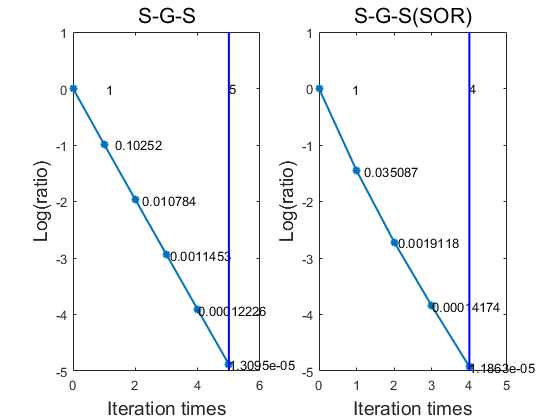
\includegraphics[width=3in]{sgs与sorsgs对比omega=1.2.png} }
		\caption{$\omega=1.2$对比}
	\end{figure}
   \indent 这里仅给出$\omega=1$与$\omega=1.2$的比较图,改变松弛因子的数值,最终发现当$\omega=1.2$左右时加速效果最好。
   \newpage
   \indent 2.对带源项的扩散方程$u_t=u_{xx}+\pi^2sin\left(\pi x\right), x\in \left[0,1\right],t\geq 0$,满足以下初始条件$u\left(x,0\right)=x^2-x$,及边界条件 $u\left(0,t\right)=u\left(1,t\right)=0$。\\
   \indent 在练习1的基础上,空间离散使用DG(P0)+DG(P0)格式,时间离散格式使用BDF1,使用LU-SGS方法在均匀网格下进行求解。
   	\vspace{10pt}\\
   \textbf{解:}\\
   \indent 与课题组练习1类似,仅改变迭代方法,这里给出单元格数为64,CFL=0.01的情况下,$U$与$U_x$的数值解与解析解的对比图,以及$U$与$U_x$的空间精度分析。\\
   \begin{figure}[!h]
   	\centering
   	\subfloat[$U$的数值解与解析解]{
   		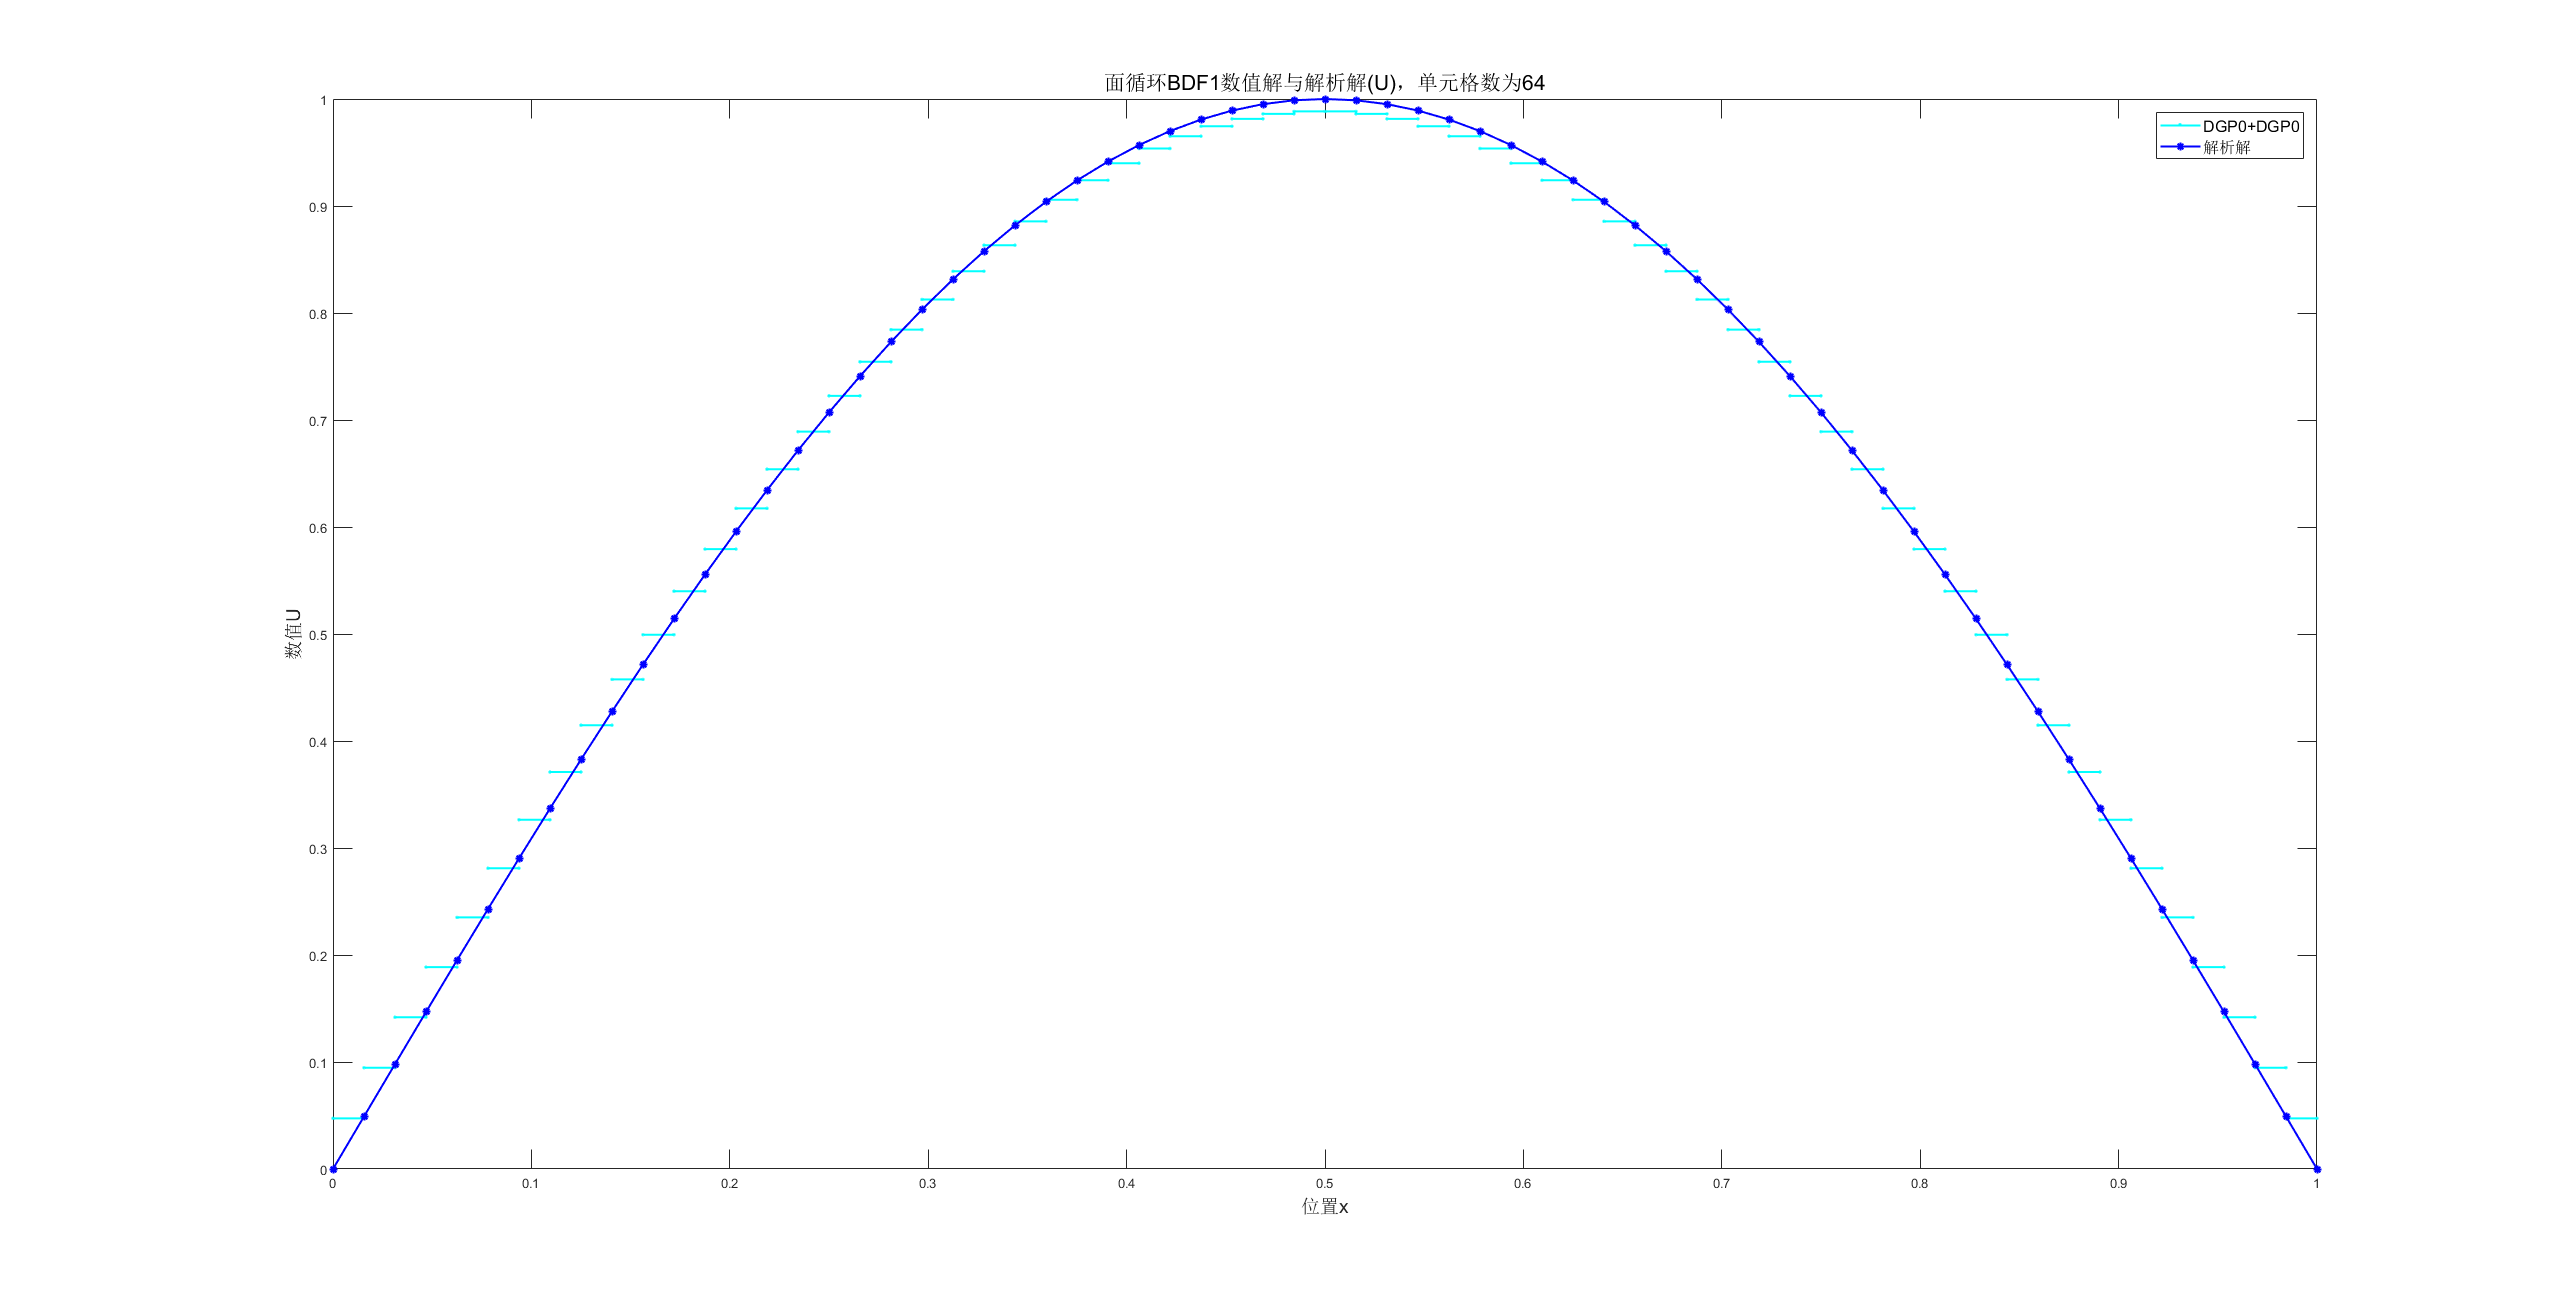
\includegraphics[width=3in]{U64.png} 
   	}
   	\hfill
   	\subfloat[$U_x$的数值解与解析解]{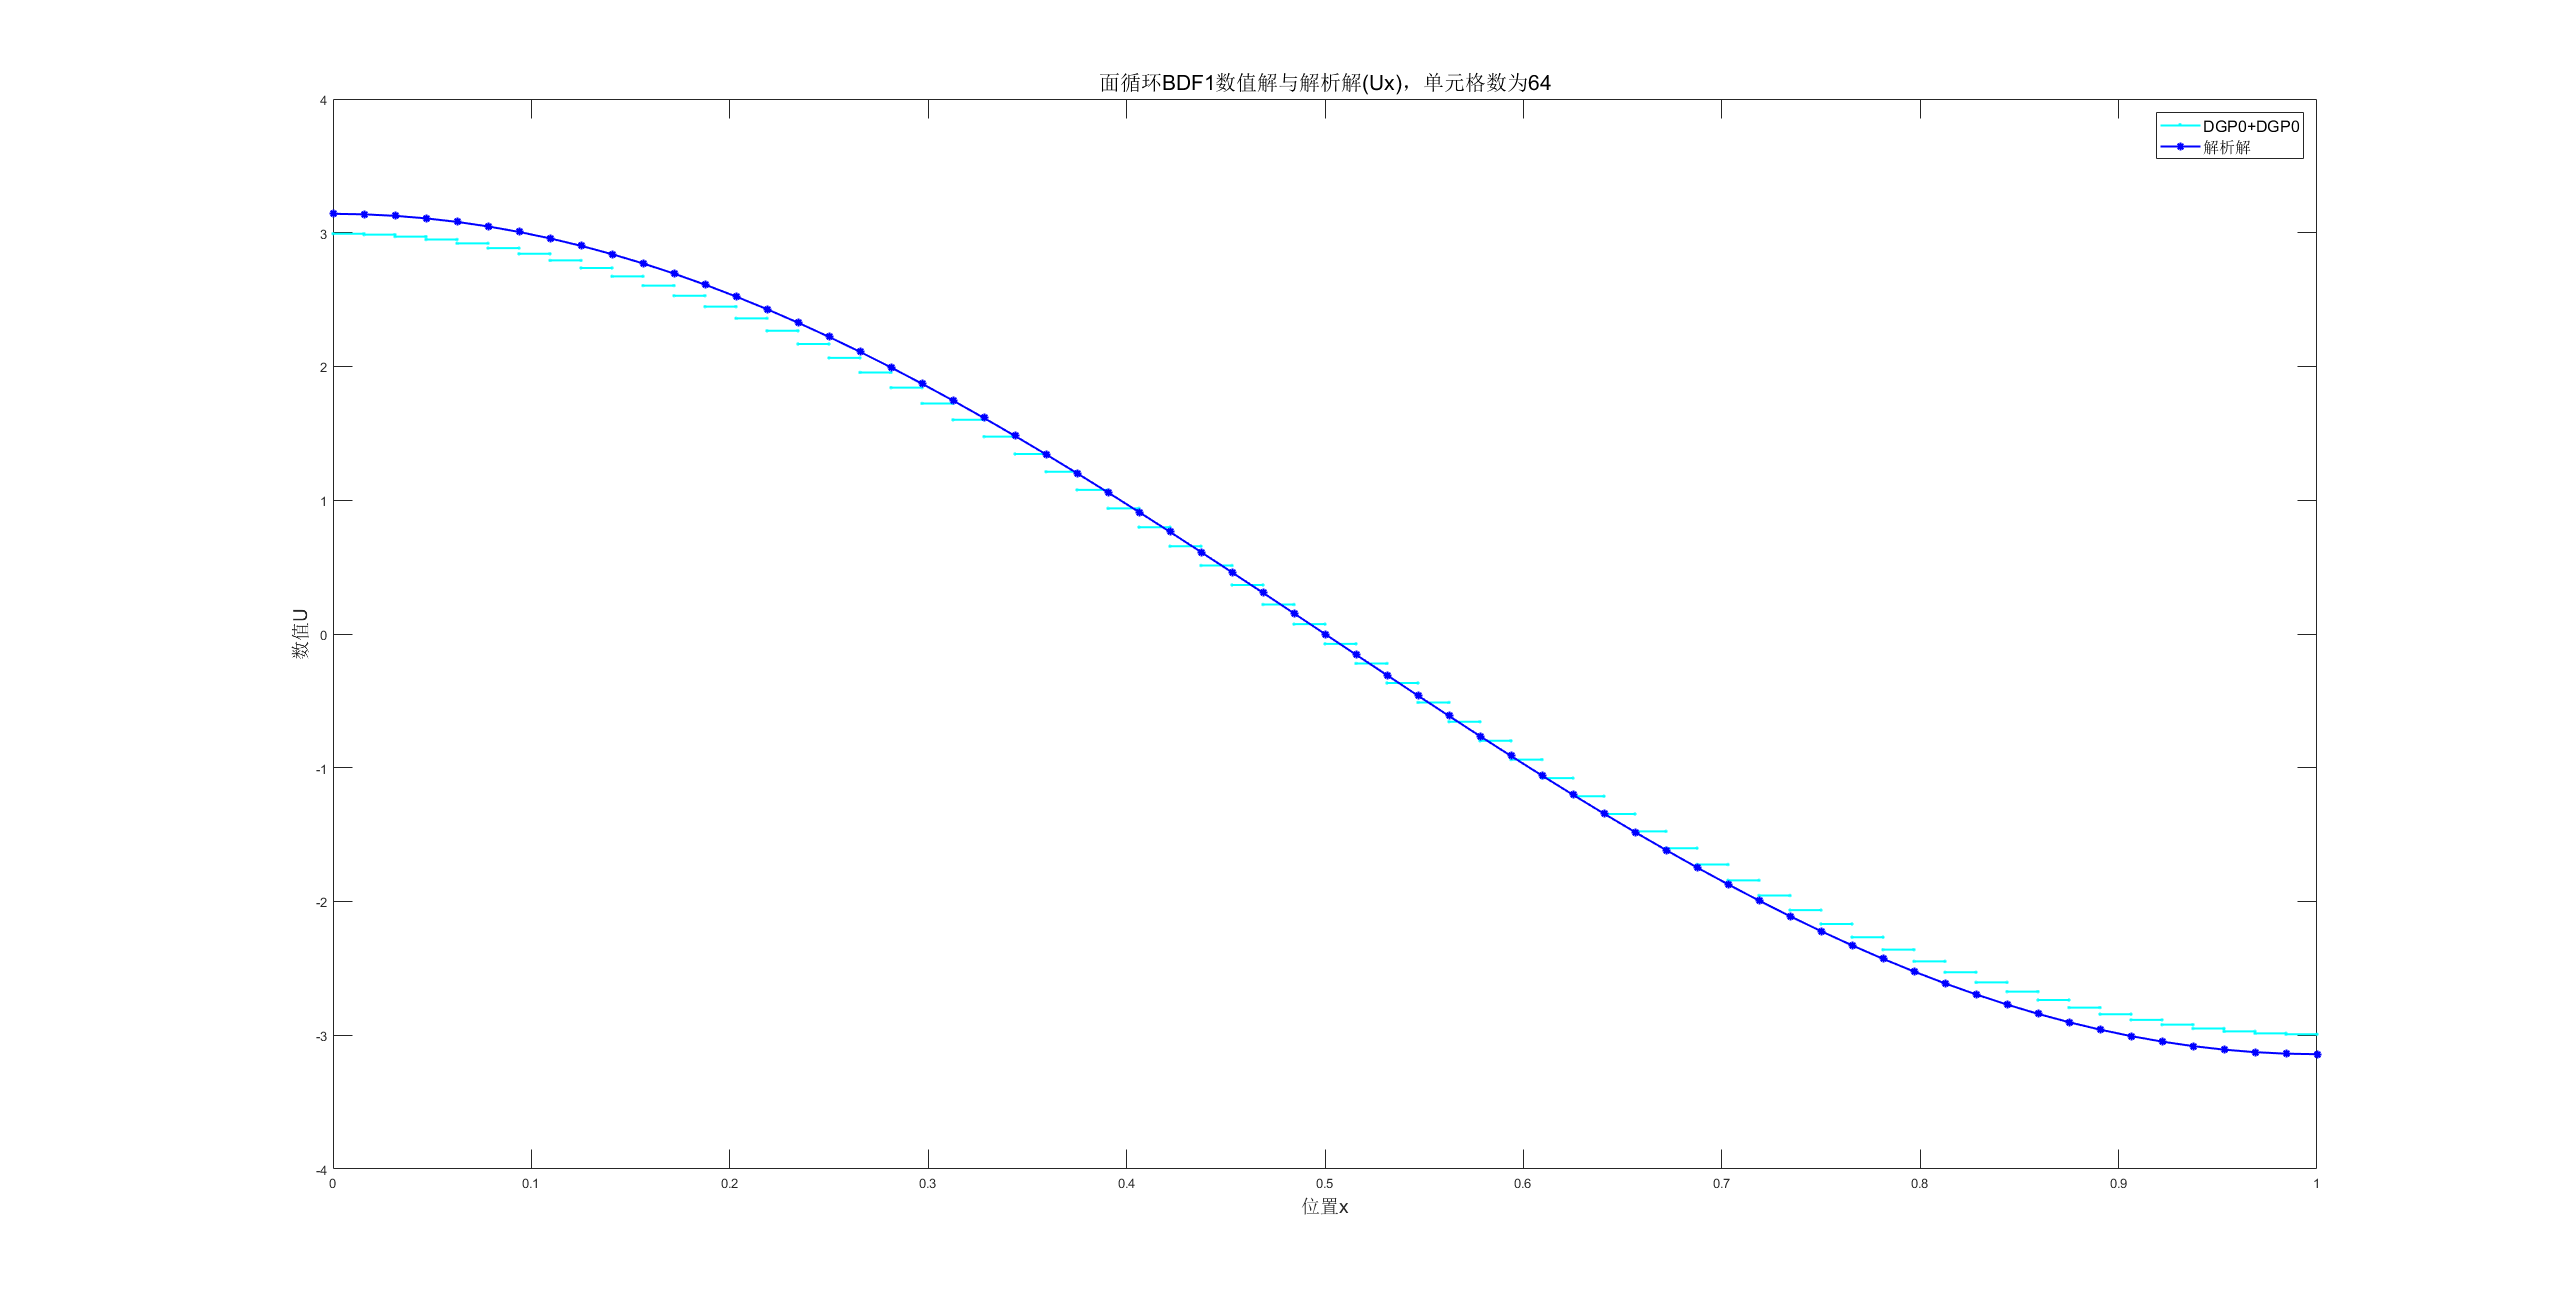
\includegraphics[width=3in]{Ux64.png} }
   	\caption{$U$与$U_x$的数值解与解析解}
   \end{figure}\\
   
   \begin{figure}[!h]
	\centering
	\subfloat[$U$的空间精度分析]{
		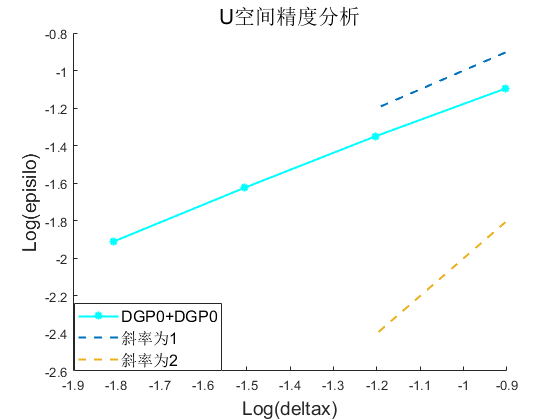
\includegraphics[width=3in]{U空间精度分析.png} 
	}
	\hfill
	\subfloat[$U_x$的空间精度分析]{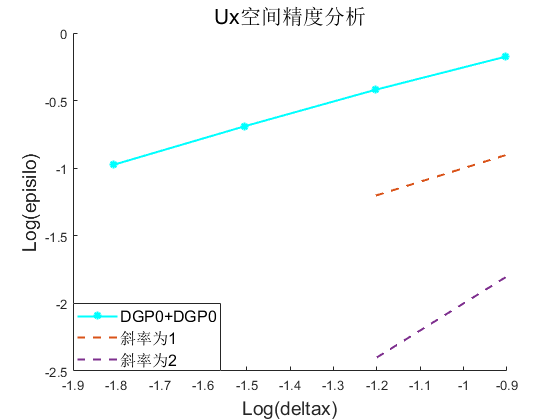
\includegraphics[width=3in]{Ux空间精度分析.png} }
	\caption{$U$与$U_x$的空间精度分析}
\end{figure}

	\clearpage
	\section{附录(代码)}
	\noindent \textbf{JacobiIteration}
	\lstset{language=Matlab}%代码语言使用的是matlab
	\lstset{breaklines}%自动将长的代码行换行排版
	\lstset{extendedchars=false}%解决代码跨页时,章节标题,页眉等汉字不显示的问题
	\begin{lstlisting}
clc
close all
clear all
% Pre-proceeding
D=3*eye(20);
L=sparse(2:20,1:19,-1/2,20,20)+sparse(3:20,1:18,-1/4,20,20);
U=L';b=100*rand(20,1);X0=rand(20,1);Xold=zeros(20,1);Xnew=zeros(20,1);
tol=10^(-5);endtimes=100;epsilon=10^(-12);
ratioR=[0:endtimes;zeros(1,endtimes+1)];
% Proceeding
Xold=X0;resnorm0=sqrt(sum(((D+L+U)*X0-b).^2))+epsilon;
resnorm=sqrt(sum(((D+L+U)*Xold-b).^2));
ratio=resnorm/resnorm0;ratioR(2,1)=ratio;
for times=2:endtimes
Xnew=-D\(L+U)*Xold+D\b;
resnorm=sqrt(sum(((D+L+U)*Xnew-b).^2));
ratio=resnorm/resnorm0;
if ratio<tol
break
end
ratioR(2,times)=ratio;
Xold=Xnew;
end
ind=find(ratioR(2,:),1,'last');
ratioR(:,ind+1:endtimes+1)=[];
plot(ratioR(1,:),log10(ratioR(2,:)),'-*','linewidth',1.5)
xlabel('Iteration times','fontsize',14)
ylabel('Log(ratio)','fontsize',14)
title('The analysis of iteration times and lgratio','fontsize',16)
hold on
str1=num2str(ratioR(2,:)');text(ratioR(1,:),log10(ratioR(2,:)),str1,'linewidth',1.5);
line([ratioR(1,ind),ratioR(1,ind)], [-5,1], 'color', 'b','linewidth',1.5);
str2=num2str(ind-1);
text(ind-1,0,str2,'linewidth',1.5);
xlim([0,ind])
	\end{lstlisting}

	\noindent \textbf{Gauss-seidelIteration}
	\begin{lstlisting}
clc
close all
clear all
% Pre-proceeding
n=20;
D=3*eye(n);
L=sparse(2:n,1:n-1,-1/2,n,n)+sparse(3:n,1:n-2,-1/4,n,n);
U=L';
A=D+L+U;
b=100*rand(n,1);b1=b;
X0=rand(n,1);XF=zeros(n,1);XB=zeros(n,1);
tol=10^(-5);endtimes=100;epsilon=10^(-12);
ratioRF=[0:endtimes;zeros(1,endtimes+1)];
ratioRB=[0:endtimes;zeros(1,endtimes+1)];
XF=X0;XB=X0;
resnorm0=sqrt(sum((A*X0-b).^2))+epsilon;
resnorm=sqrt(sum((A*XF-b).^2));
ratio=resnorm/resnorm0;ratioRF(2,1)=ratio;ratioRB(2,1)=ratio;

% Proceeding
%Forward sweep
for times=2:endtimes
%calculate X
for i=1:n
for j=1:i-1
b(i)=b(i)-A(i,j)*XF(j);
end
for j=i+1:n
b(i)=b(i)-A(i,j)*XF(j);
end
XF(i)=b(i)/A(i,i);
end
b=b1;
resnorm=sqrt(sum((A*XF-b).^2));
ratio=resnorm/resnorm0;
if ratio<tol
break
end
ratioRF(2,times)=ratio;
end
ind=find(ratioRF(2,:),1,'last');
ratioRF(:,ind+1:endtimes+1)=[];
subplot(1,2,1)
plot(ratioRF(1,:),log10(ratioRF(2,:)),'-*','linewidth',1.5)
xlabel('Iteration times','fontsize',14)
ylabel('Log(ratio)','fontsize',14)
title('G-S Forward sweep','fontsize',16)
hold on
str1=num2str(ratioRF(2,:)');text(ratioRF(1,:),log10(ratioRF(2,:)),str1,'linewidth',1.5);
line([ratioRF(1,ind),ratioRF(1,ind)], [-5,1], 'color', 'b','linewidth',1.5);
str2=num2str(ind-1);
text(ind-1,0,str2,'linewidth',1.5);
xlim([0,ind])


%Backward sweep
for times=2:endtimes
%calculate X
for i=n:-1:1
for j=n:-1:i+1
b(i)=b(i)-A(i,j)*XB(j);
end
for j=i-1:-1:1
b(i)=b(i)-A(i,j)*XB(j);
end
XB(i)=b(i)/A(i,i);
end
b=b1;
resnorm=sqrt(sum((A*XB-b).^2));
ratio=resnorm/resnorm0;
if ratio<tol
break
end
ratioRB(2,times)=ratio;
end
ind=find(ratioRB(2,:),1,'last');
ratioRB(:,ind+1:endtimes+1)=[];
subplot(1,2,2)
plot(ratioRB(1,:),log10(ratioRB(2,:)),'-*','linewidth',1.5)
xlabel('Iteration times','fontsize',14)
ylabel('Log(ratio)','fontsize',14)
title('G-S Backward sweep','fontsize',16)
hold on
str1=num2str(ratioRB(2,:)');text(ratioRB(1,:),log10(ratioRB(2,:)),str1,'linewidth',1.5);
line([ratioRB(1,ind),ratioRB(1,ind)], [-5,1], 'color', 'b','linewidth',1.5);
str2=num2str(ind-1);
text(ind-1,0,str2,'linewidth',1.5);
xlim([0,ind])
	\end{lstlisting}

\noindent \textbf{S-G(SOR) and S-G-S(SOR)}
\lstset{language=Matlab}%代码语言使用的是matlab
\lstset{breaklines}%自动将长的代码行换行排版
\lstset{extendedchars=false}%解决代码跨页时,章节标题,页眉等汉字不显示的问题
\begin{lstlisting}
clc
close all
clear all
% Pre-proceeding
n=20;
omega=1;%松弛因子
%构建矩阵
D=3*eye(n);
L=sparse(2:n,1:n-1,-1/2,n,n)+sparse(3:n,1:n-2,-1/4,n,n);
U=L';
A=D+L+U;
b=[1:n]';b1=b;
X0=zeros(n,1);XF=zeros(n,1);Xsgs=zeros(n,1);Xold=zeros(n,1);
%终止条件等
tol=10^(-5);endtimes=100;epsilon=10^(-12);
ratioRF=[0:endtimes;zeros(1,endtimes+1)];
ratioRsgs=[0:endtimes;zeros(1,endtimes+1)];
ratioRSORFGS=[0:endtimes;zeros(1,endtimes+1)];
ratioRSORSGS=[0:endtimes;zeros(1,endtimes+1)];
XF=X0;Xsgs=X0;Xsorfgs=X0;Xsorsgs=X0;
resnorm0=sqrt(sum((A*X0-b).^2))+epsilon;
resnorm=sqrt(sum((A*XF-b).^2));
ratio=resnorm/resnorm0;ratioRF(2,1)=ratio;ratioRsgs(2,1)=ratio;ratioRSORFGS(2,1)=ratio;ratioRSORSGS(2,1)=ratio;

% Proceeding
%G-S-Forward sweep
for times=2:endtimes
%calculate X
for i=1:n
for j=1:i-1
b(i)=b(i)-A(i,j)*XF(j);
end
for j=i+1:n
b(i)=b(i)-A(i,j)*XF(j);
end
XF(i)=b(i)/A(i,i);
end
b=b1;
resnorm=sqrt(sum((A*XF-b).^2));
ratio=resnorm/resnorm0;
if ratio<tol
break
end
ratioRF(2,times)=ratio;
end
ind=find(ratioRF(2,:),1,'last');
ratioRF(:,ind+1:endtimes+1)=[];
subplot(1,2,1)
plot(ratioRF(1,:),log10(ratioRF(2,:)),'-*','linewidth',1.5)
xlabel('Iteration times','fontsize',14)
ylabel('Log(ratio)','fontsize',14)
title('G-S Forward sweep','fontsize',16)
hold on
str1=num2str(ratioRF(2,:)');text(ratioRF(1,:),log10(ratioRF(2,:)),str1,'linewidth',1.5);
line([ratioRF(1,ind),ratioRF(1,ind)], [-5,1], 'color', 'b','linewidth',1.5);
str2=num2str(ind-1);
text(ind-1,0,str2,'linewidth',1.5);
xlim([0,ind])

%SOR-FGS 
R=b1-A*X0;
for times=2:endtimes
%calculate deltaX
Xold=Xsorfgs;
ie=1;
Xsorfgs(ie)=R(ie)/(D(ie,ie)/omega);
ie=2;
R(ie)=R(ie)-Xsorfgs(ie-1)*(L(ie,ie-1)/omega);
Xsorfgs(ie)=R(ie)/(D(ie,ie)/omega);
for ie=3:n
R(ie)=R(ie)-Xsorfgs(ie-1)*(L(ie,ie-1)/omega)-Xsorfgs(ie-2)*(L(ie,ie-2)/omega);
Xsorfgs(ie)=R(ie)/(D(ie,ie)/omega);
end
Xsorfgs=Xsorfgs+Xold;
resnorm=sqrt(sum((A*Xsorfgs-b1).^2));
ratio=resnorm/resnorm0;
if ratio<tol
break
end
R=b1-A*Xsorfgs;
ratioRSORFGS(2,times)=ratio;
end
ind=find(ratioRSORFGS(2,:),1,'last');
ratioRSORFGS(:,ind+1:endtimes+1)=[];
subplot(1,2,2)
plot(ratioRSORFGS(1,:),log10(ratioRSORFGS(2,:)),'-*','linewidth',1.5)
xlabel('Iteration times','fontsize',14)
ylabel('Log(ratio)','fontsize',14)
title('G-S Forward sweep(SOR)','fontsize',16)
hold on
str1=num2str(ratioRSORFGS(2,:)');text(ratioRSORFGS(1,:),log10(ratioRSORFGS(2,:)),str1,'linewidth',1.5);
line([ratioRSORFGS(1,ind),ratioRSORFGS(1,ind)], [-5,1], 'color', 'b','linewidth',1.5);
str2=num2str(ind-1);
text(ind-1,0,str2,'linewidth',1.5);
xlim([0,ind])

%SGS
for times=2:endtimes
%calculate X Forward sweep
for i=1:n
for j=1:i-1
b(i)=b(i)-A(i,j)*Xsgs(j);
end
for j=i+1:n
b(i)=b(i)-A(i,j)*Xsgs(j);
end
Xsgs(i)=b(i)/A(i,i);
end
b=b1;
%Backward sweep
for i=n:-1:1
for j=n:-1:i+1
b(i)=b(i)-A(i,j)*Xsgs(j);
end
for j=i-1:-1:1
b(i)=b(i)-A(i,j)*Xsgs(j);
end
Xsgs(i)=b(i)/A(i,i);
end
b=b1;
resnorm=sqrt(sum((A*Xsgs-b).^2));
ratio=resnorm/resnorm0;
if ratio<tol
break
end
ratioRsgs(2,times)=ratio;
end
ind=find(ratioRsgs(2,:),1,'last');
ratioRsgs(:,ind+1:endtimes+1)=[];
figure
subplot(1,2,1)
plot(ratioRsgs(1,:),log10(ratioRsgs(2,:)),'-*','linewidth',1.5)
xlabel('Iteration times','fontsize',14)
ylabel('Log(ratio)','fontsize',14)
title('S-G-S','fontsize',16)
hold on
str1=num2str(ratioRsgs(2,:)');text(ratioRsgs(1,:),log10(ratioRsgs(2,:)),str1,'linewidth',1.5);
line([ratioRsgs(1,ind),ratioRsgs(1,ind)], [-5,1], 'color', 'b','linewidth',1.5);
str2=num2str(ind-1);
text(ind-1,0,str2,'linewidth',1.5);
xlim([0,ind])
hold off


%SOR-SGS
R=omega*(2-omega)*(b1-A*X0);
for times=2:endtimes
%calculate deltaX   
%Forward sweep
Xold=Xsorsgs;
ie=1;
Xsorsgs(ie)=R(ie)/D(ie,ie);
ie=2;
R(ie)=R(ie)-Xsorsgs(ie-1)*(L(ie,ie-1)*omega);
Xsorsgs(ie)=R(ie)/D(ie,ie);
for ie=3:n
R(ie)=R(ie)-Xsorsgs(ie-1)*(L(ie,ie-1)*omega)-Xsorsgs(ie-2)*(L(ie,ie-2)*omega);
Xsorsgs(ie)=R(ie)/D(ie,ie);
end
%Backward sweep
R=D*Xsorsgs;
ie=n;
Xsorsgs(ie)=R(ie)/D(ie,ie);
ie=n-1;
R(ie)=R(ie)-Xsorsgs(ie+1)*(U(ie,ie+1)*omega);
Xsorsgs(ie)=R(ie)/D(ie,ie);
for ie=n-2:-1:1
R(ie)=R(ie)-Xsorsgs(ie+1)*(U(ie,ie+1)*omega)-Xsorsgs(ie+2)*(U(ie,ie+2)*omega);
Xsorsgs(ie)=R(ie)/D(ie,ie);
end
%此时Xsorsgs里面存储的是deltaX
Xsorsgs=Xsorsgs+Xold;
resnorm=sqrt(sum((A*Xsorsgs-b1).^2));
ratio=resnorm/resnorm0;
if ratio<tol
break
end
R=omega*(2-omega)*(b1-A*Xsorsgs);
ratioRSORSGS(2,times)=ratio;
end
ind=find(ratioRSORSGS(2,:),1,'last');
ratioRSORSGS(:,ind+1:endtimes+1)=[];
subplot(1,2,2)
plot(ratioRSORSGS(1,:),log10(ratioRSORSGS(2,:)),'-*','linewidth',1.5)
xlabel('Iteration times','fontsize',14)
ylabel('Log(ratio)','fontsize',14)
title('S-G-S(SOR)','fontsize',16)
hold on
str1=num2str(ratioRSORSGS(2,:)');text(ratioRSORSGS(1,:),log10(ratioRSORSGS(2,:)),str1,'linewidth',1.5);
line([ratioRSORSGS(1,ind),ratioRSORSGS(1,ind)], [-5,1], 'color', 'b','linewidth',1.5);
str2=num2str(ind-1);
text(ind-1,0,str2,'linewidth',1.5);
xlim([0,ind])
\end{lstlisting}
	
	\noindent \textbf{subDG(P0)+DG(P0) L-U Iteration}
\begin{lstlisting}
function [Unumsolution,n]=subDGP0plusDGP0(Unit,CFL,endtau)
%Some basic paramater
endx=1;deltax=endx/Unit;numberx=endx/deltax+1;
tol=10^(-10);
nu=1;Lr=1/(2*pi);Tr=Lr^2/nu;
abslambda=sqrt(nu/Tr);deltatau=CFL*deltax/abslambda;%伪时间变量
B1=1;
C=[B1,0;0,B1/deltax];Mtau=[deltax,0;0,1/deltax];%此为推导出的U=CV中的C
A=[abslambda,0;0,abslambda];epsilon=10^(-12);
R=zeros(2*Unit,1);
Rd=zeros(2,numberx-1);
Rb=zeros(2,numberx-1);
Fn=zeros(2,numberx);
X=zeros(2*Unit,1);


%构建LHS
%Mtau/deltatau
LHS1=sparse(1:2:2*Unit-1,1:2:2*Unit-1,deltax/deltatau,2*Unit,2*Unit);
LHS1=LHS1+sparse(2:2:2*Unit,2:2:2*Unit,1/(deltax*deltatau),2*Unit,2*Unit);
%Rdomain
LHS2=-sparse(2:2:2*Unit,2:2:2*Unit,-1/(Tr*deltax),2*Unit,2*Unit);
%Rboundary
LHS3=zeros(2*Unit,2*Unit);
for iface=2:numberx-1
ieL=iface-1;
ieR=iface;
%diag
LHS3(2*ieL-1:2*ieL,2*ieL-1:2*ieL)=LHS3(2*ieL-1:2*ieL,2*ieL-1:2*ieL)+C'*[abslambda/2,-nu/(2*deltax);-1/(2*Tr),abslambda/(2*deltax)];
LHS3(2*ieR-1:2*ieR,2*ieR-1:2*ieR)=LHS3(2*ieR-1:2*ieR,2*ieR-1:2*ieR)-C'*[-abslambda/2,-nu/(2*deltax);-1/(2*Tr),-abslambda/(2*deltax)];
%upper
LHS3(2*ieL-1:2*ieL,2*ieR-1:2*ieR)=LHS3(2*ieL-1:2*ieL,2*ieR-1:2*ieR)+C'*[-abslambda/2,-nu/(2*deltax);-1/(2*Tr),-abslambda/(2*deltax)];
%lower
LHS3(2*ieR-1:2*ieR,2*ieL-1:2*ieL)=LHS3(2*ieR-1:2*ieR,2*ieL-1:2*ieL)-C'*[abslambda/2,-nu/(2*deltax);-1/(2*Tr),abslambda/(2*deltax)];
end
LHS3(2*1-1:2*1,2*1-1:2*1)=LHS3(2*1-1:2*1,2*1-1:2*1)-C'*([abslambda/2,-nu/2;-1/(2*Tr),abslambda/2]*[0,0;0,1]+[-abslambda/2,-nu/2;-1/(2*Tr),-abslambda/2])*C;
LHS3(2*(numberx-1)-1:2*(numberx-1),2*(numberx-1)-1:2*(numberx-1))=LHS3(2*(numberx-1)-1:2*(numberx-1),2*(numberx-1)-1:2*(numberx-1))+C'*([abslambda/2,-nu/2;-1/(2*Tr),abslambda/2]+[-abslambda/2,-nu/2;-1/(2*Tr),-abslambda/2]*[0,0;0,1])*C;

LHS=LHS1+LHS2+LHS3;

%取出我们所需要的D
D=zeros(2*Unit,2*Unit);
for iface=2:numberx
ieL=iface-1;
D(2*ieL-1:2*ieL,2*ieL-1:2*ieL)=LHS(2*ieL-1:2*ieL,2*ieL-1:2*ieL);
end
%取出我们所需要的L
L=zeros(2*Unit,2*Unit);
for iface=2:numberx-1
ieR=iface;
ieL=iface-1;
L(2*ieR-1:2*ieR,2*ieL-1:2*ieL)=LHS(2*ieR-1:2*ieR,2*ieL-1:2*ieL);
end

%取出我们所需要的U
U=zeros(2*Unit,2*Unit);
for iface=2:numberx-1
ieR=iface;
ieL=iface-1;
U(2*ieL-1:2*ieL,2*ieR-1:2*ieR)= LHS(2*ieL-1:2*ieL,2*ieR-1:2*ieR);
end


%为循环所预设的一些量

Ucurrent=zeros(2,numberx-1);
Unext=zeros(2*Unit,1);
%initial  condition set up
x=0;

for k=1:numberx-1
Ucurrent(1,k)=(x+deltax/2)^2-(x+deltax/2);
Ucurrent(2,k)=(2*(x+deltax/2)-1)*deltax;
x=x+deltax;
end

%Rdomain
x=0;
for k=1:numberx-1
Rd(1,k)=pi*(cos(pi*x)-cos(pi*(x+deltax)));
Rd(2,k)=-Ucurrent(2,k)/(Tr*deltax);
x=x+deltax;
end
%Rboundary
for iface=2:numberx-1
ieL=iface-1;
ieR=iface;
Fn(:,iface)=0.5*([-nu*Ucurrent(2,ieL)/deltax;-Ucurrent(1,ieL)/Tr]+[-nu*Ucurrent(2,ieR)/deltax;-Ucurrent(1,ieR)/Tr])-0.5*A*([Ucurrent(1,ieR);Ucurrent(2,ieR)/deltax]-[Ucurrent(1,ieL);Ucurrent(2,ieL)/deltax]);
Rb(:,ieL)=Rb(:,ieL)-C'*Fn(:,iface);
Rb(:,ieR)=Rb(:,ieR)+C'*Fn(:,iface);
end
Fn(:,1)=0.5*([-nu*Ucurrent(2,1)/deltax;0]+[-nu*Ucurrent(2,1)/deltax;-Ucurrent(1,1)/Tr])-0.5*A*([Ucurrent(1,1);Ucurrent(2,1)/deltax]-[0;Ucurrent(2,1)/deltax]);
Fn(:,numberx)=0.5*([-nu*Ucurrent(2,numberx-1)/deltax;-Ucurrent(1,numberx-1)/Tr]+[-nu*Ucurrent(2,numberx-1)/deltax;0])-0.5*A*([0;Ucurrent(2,numberx-1)/deltax]-[Ucurrent(1,numberx-1);Ucurrent(2,numberx-1)/deltax]);
Rb(:,1)=Rb(:,1)+C'*Fn(:,1);
Rb(:,numberx-1)=Rb(:,numberx-1)-C'*Fn(:,numberx);

%R组装
for k=1:numberx-1
R(2*k-1:2*k,1)=Rd(:,k)+Rb(:,k);
end
%进行必要的向量等价转变
for k=1:numberx-1
Unext(2*k-1:2*k,1)=Ucurrent(:,k);
end

%循环迭代
for n=deltatau:deltatau:endtau
X=0;
b=R;
%Forward sweep
ie=1;
X(ie:ie+1,1)=D(ie:ie+1,ie:ie+1)\R(ie:ie+1,1);
for ie=2:numberx-1
R(2*ie-1:2*ie,1)=R(2*ie-1:2*ie,1)-L(2*ie-1:2*ie,2*(ie-1)-1:2*(ie-1))*X(2*(ie-1)-1:2*(ie-1),1);
X(2*ie-1:2*ie,1)=D(2*ie-1:2*ie,2*ie-1:2*ie)\R(2*ie-1:2*ie,1);
end
%Backward sweep
for ie=1:numberx-1
R(2*ie-1:2*ie,1)= D(2*ie-1:2*ie,2*ie-1:2*ie)*X(2*ie-1:2*ie,1);
end

ie=numberx-1;
X(2*ie-1:2*ie)=D(2*ie-1:2*ie,2*ie-1:2*ie)\R(2*ie-1:2*ie,1);
for ie=numberx-2:-1:1
R(2*ie-1:2*ie,1)=R(2*ie-1:2*ie,1)-U(2*ie-1:2*ie,2*(ie+1)-1:2*(ie+1))*X(2*(ie+1)-1:2*(ie+1),1);
X(2*ie-1:2*ie,1)=D(2*ie-1:2*ie,2*ie-1:2*ie)\R(2*ie-1:2*ie,1);
end
if max(X)<tol
break
end
Unext=Unext+X;
Rd=zeros(2,numberx-1);
Rb=zeros(2,numberx-1);    
for k=1:numberx-1
Ucurrent(:,k)=Unext(2*k-1:2*k,1);
end
%Rdomain
x=0;
for k=1:numberx-1
Rd(1,k)=pi*(cos(pi*x)-cos(pi*(x+deltax)));
Rd(2,k)=-Ucurrent(2,k)/(Tr*deltax);
x=x+deltax;
end
%Rboundary
for iface=2:numberx-1
ieL=iface-1;
ieR=iface;
Fn(:,iface)=0.5*([-nu*Ucurrent(2,ieL)/deltax;-Ucurrent(1,ieL)/Tr]+[-nu*Ucurrent(2,ieR)/deltax;-Ucurrent(1,ieR)/Tr])-0.5*A*([Ucurrent(1,ieR);Ucurrent(2,ieR)/deltax]-[Ucurrent(1,ieL);Ucurrent(2,ieL)/deltax]);
Rb(:,ieL)=Rb(:,ieL)-C'*Fn(:,iface);
Rb(:,ieR)=Rb(:,ieR)+C'*Fn(:,iface);
end

Fn(:,1)=0.5*([-nu*Ucurrent(2,1)/deltax;0]+[-nu*Ucurrent(2,1)/deltax;-Ucurrent(1,1)/Tr])-0.5*A*([Ucurrent(1,1);Ucurrent(2,1)/deltax]-[0;Ucurrent(2,1)/deltax]);
Fn(:,numberx)=0.5*([-nu*Ucurrent(2,numberx-1)/deltax;-Ucurrent(1,numberx-1)/Tr]+[-nu*Ucurrent(2,numberx-1)/deltax;0])-0.5*A*([0;Ucurrent(2,numberx-1)/deltax]-[Ucurrent(1,numberx-1);Ucurrent(2,numberx-1)/deltax]);
Rb(:,1)=Rb(:,1)+C'*Fn(:,1);
Rb(:,numberx-1)=Rb(:,numberx-1)-C'*Fn(:,numberx);

%R组装
for k=1:numberx-1
R(2*k-1:2*k,1)=Rd(:,k)+Rb(:,k);
end

for k=1:numberx-1
Unext(2*k-1:2*k,1)=Ucurrent(:,k);
end
end
Unumsolution(1,:)=Ucurrent(1,:);Unumsolution(2,:)=Ucurrent(2,:)/deltax;
end

\end{lstlisting}


	
\end{document}